\documentclass[twoside]{book}

% Packages required by doxygen
\usepackage{fixltx2e}
\usepackage{calc}
\usepackage{doxygen}
\usepackage{graphicx}
\usepackage[utf8]{inputenc}
\usepackage{makeidx}
\usepackage{multicol}
\usepackage{multirow}
\PassOptionsToPackage{warn}{textcomp}
\usepackage{textcomp}
\usepackage[nointegrals]{wasysym}
\usepackage[table]{xcolor}

% NLS support packages
\usepackage[T2A]{fontenc}
\usepackage[russian]{babel}

% Font selection
\usepackage[T1]{fontenc}
\usepackage{mathptmx}
\usepackage[scaled=.90]{helvet}
\usepackage{courier}
\usepackage{amssymb}
\usepackage{sectsty}
\renewcommand{\familydefault}{\sfdefault}
\allsectionsfont{%
  \fontseries{bc}\selectfont%
  \color{darkgray}%
}
\renewcommand{\DoxyLabelFont}{%
  \fontseries{bc}\selectfont%
  \color{darkgray}%
}
\newcommand{\+}{\discretionary{\mbox{\scriptsize$\hookleftarrow$}}{}{}}

% Page & text layout
\usepackage{geometry}
\geometry{%
  a4paper,%
  top=2.5cm,%
  bottom=2.5cm,%
  left=2.5cm,%
  right=2.5cm%
}
\tolerance=750
\hfuzz=15pt
\hbadness=750
\setlength{\emergencystretch}{15pt}
\setlength{\parindent}{0cm}
\setlength{\parskip}{0.2cm}
\makeatletter
\renewcommand{\paragraph}{%
  \@startsection{paragraph}{4}{0ex}{-1.0ex}{1.0ex}{%
    \normalfont\normalsize\bfseries\SS@parafont%
  }%
}
\renewcommand{\subparagraph}{%
  \@startsection{subparagraph}{5}{0ex}{-1.0ex}{1.0ex}{%
    \normalfont\normalsize\bfseries\SS@subparafont%
  }%
}
\makeatother

% Headers & footers
\usepackage{fancyhdr}
\pagestyle{fancyplain}
\fancyhead[LE]{\fancyplain{}{\bfseries\thepage}}
\fancyhead[CE]{\fancyplain{}{}}
\fancyhead[RE]{\fancyplain{}{\bfseries\leftmark}}
\fancyhead[LO]{\fancyplain{}{\bfseries\rightmark}}
\fancyhead[CO]{\fancyplain{}{}}
\fancyhead[RO]{\fancyplain{}{\bfseries\thepage}}
\fancyfoot[LE]{\fancyplain{}{}}
\fancyfoot[CE]{\fancyplain{}{}}
\fancyfoot[RE]{\fancyplain{}{\bfseries\scriptsize Документация по Viselitsa. Последние изменения\+: Пт 10 Май 2024 20\+:28\+:55. Создано системой Doxygen }}
\fancyfoot[LO]{\fancyplain{}{\bfseries\scriptsize Документация по Viselitsa. Последние изменения\+: Пт 10 Май 2024 20\+:28\+:55. Создано системой Doxygen }}
\fancyfoot[CO]{\fancyplain{}{}}
\fancyfoot[RO]{\fancyplain{}{}}
\renewcommand{\footrulewidth}{0.4pt}
\renewcommand{\chaptermark}[1]{%
  \markboth{#1}{}%
}
\renewcommand{\sectionmark}[1]{%
  \markright{\thesection\ #1}%
}

% Indices & bibliography
\usepackage{natbib}
\usepackage[titles]{tocloft}
\setcounter{tocdepth}{3}
\setcounter{secnumdepth}{5}
\makeindex

% Hyperlinks (required, but should be loaded last)
\usepackage{ifpdf}
\ifpdf
  \usepackage[pdftex,pagebackref=true]{hyperref}
\else
  \usepackage[ps2pdf,pagebackref=true]{hyperref}
\fi
\hypersetup{%
  colorlinks=true,%
  linkcolor=blue,%
  citecolor=blue,%
  unicode%
}

% Custom commands
\newcommand{\clearemptydoublepage}{%
  \newpage{\pagestyle{empty}\cleardoublepage}%
}


%===== C O N T E N T S =====

\begin{document}

% Titlepage & ToC
\hypersetup{pageanchor=false,
             bookmarks=true,
             bookmarksnumbered=true,
             pdfencoding=unicode
            }
\pagenumbering{roman}
\begin{titlepage}
\vspace*{7cm}
\begin{center}%
{\Large Viselitsa \\[1ex]\large 1.\+1.\+20 }\\
\vspace*{1cm}
{\large Создано системой Doxygen 1.8.8}\\
\vspace*{0.5cm}
{\small Пт 10 Май 2024 20:28:55}\\
\end{center}
\end{titlepage}
\clearemptydoublepage
\tableofcontents
\clearemptydoublepage
\pagenumbering{arabic}
\hypersetup{pageanchor=true}

%--- Begin generated contents ---
\chapter{Алфавитный указатель пространств имен}
\section{Пространства имен}
Полный список документированных пространств имен.\begin{DoxyCompactList}
\item\contentsline{section}{\hyperlink{namespace_xD0_x92_xD0_xB8_xD1_x81_xD0_xB5_xD0_xBB_xD0_xB8_xD1_x86_xD0_xB0}{Виселица} }{\pageref{namespace_xD0_x92_xD0_xB8_xD1_x81_xD0_xB5_xD0_xBB_xD0_xB8_xD1_x86_xD0_xB0}}{}
\end{DoxyCompactList}

\chapter{Иерархический список классов}
\section{Иерархия классов}
Иерархия классов.\begin{DoxyCompactList}
\item Form\begin{DoxyCompactList}
\item \contentsline{section}{Виселица.\+Difficulty\+Animals}{\pageref{class_xD0_x92_xD0_xB8_xD1_x81_xD0_xB5_xD0_xBB_xD0_xB8_xD1_x86_xD0_xB0_1_1_difficulty_animals}}{}
\item \contentsline{section}{Виселица.\+Difficulty\+Cities}{\pageref{class_xD0_x92_xD0_xB8_xD1_x81_xD0_xB5_xD0_xBB_xD0_xB8_xD1_x86_xD0_xB0_1_1_difficulty_cities}}{}
\item \contentsline{section}{Виселица.\+Difficulty\+Countries}{\pageref{class_xD0_x92_xD0_xB8_xD1_x81_xD0_xB5_xD0_xBB_xD0_xB8_xD1_x86_xD0_xB0_1_1_difficulty_countries}}{}
\item \contentsline{section}{Виселица.\+Game\+Average\+Animals}{\pageref{class_xD0_x92_xD0_xB8_xD1_x81_xD0_xB5_xD0_xBB_xD0_xB8_xD1_x86_xD0_xB0_1_1_game_average_animals}}{}
\item \contentsline{section}{Виселица.\+Game\+Average\+Cities}{\pageref{class_xD0_x92_xD0_xB8_xD1_x81_xD0_xB5_xD0_xBB_xD0_xB8_xD1_x86_xD0_xB0_1_1_game_average_cities}}{}
\item \contentsline{section}{Виселица.\+Game\+Average\+Countries}{\pageref{class_xD0_x92_xD0_xB8_xD1_x81_xD0_xB5_xD0_xBB_xD0_xB8_xD1_x86_xD0_xB0_1_1_game_average_countries}}{}
\item \contentsline{section}{Виселица.\+Game\+Difficult\+Animals}{\pageref{class_xD0_x92_xD0_xB8_xD1_x81_xD0_xB5_xD0_xBB_xD0_xB8_xD1_x86_xD0_xB0_1_1_game_difficult_animals}}{}
\item \contentsline{section}{Виселица.\+Game\+Difficult\+Cities}{\pageref{class_xD0_x92_xD0_xB8_xD1_x81_xD0_xB5_xD0_xBB_xD0_xB8_xD1_x86_xD0_xB0_1_1_game_difficult_cities}}{}
\item \contentsline{section}{Виселица.\+Game\+Difficult\+Countries}{\pageref{class_xD0_x92_xD0_xB8_xD1_x81_xD0_xB5_xD0_xBB_xD0_xB8_xD1_x86_xD0_xB0_1_1_game_difficult_countries}}{}
\item \contentsline{section}{Виселица.\+Game\+Light\+Animals}{\pageref{class_xD0_x92_xD0_xB8_xD1_x81_xD0_xB5_xD0_xBB_xD0_xB8_xD1_x86_xD0_xB0_1_1_game_light_animals}}{}
\item \contentsline{section}{Виселица.\+Game\+Light\+Cities}{\pageref{class_xD0_x92_xD0_xB8_xD1_x81_xD0_xB5_xD0_xBB_xD0_xB8_xD1_x86_xD0_xB0_1_1_game_light_cities}}{}
\item \contentsline{section}{Виселица.\+Game\+Light\+Countries}{\pageref{class_xD0_x92_xD0_xB8_xD1_x81_xD0_xB5_xD0_xBB_xD0_xB8_xD1_x86_xD0_xB0_1_1_game_light_countries}}{}
\item \contentsline{section}{Виселица.\+Menu}{\pageref{class_xD0_x92_xD0_xB8_xD1_x81_xD0_xB5_xD0_xBB_xD0_xB8_xD1_x86_xD0_xB0_1_1_menu}}{}
\item \contentsline{section}{Виселица.\+Player}{\pageref{class_xD0_x92_xD0_xB8_xD1_x81_xD0_xB5_xD0_xBB_xD0_xB8_xD1_x86_xD0_xB0_1_1_player}}{}
\item \contentsline{section}{Виселица.\+Spravka}{\pageref{class_xD0_x92_xD0_xB8_xD1_x81_xD0_xB5_xD0_xBB_xD0_xB8_xD1_x86_xD0_xB0_1_1_spravka}}{}
\item \contentsline{section}{Виселица.\+Table}{\pageref{class_xD0_x92_xD0_xB8_xD1_x81_xD0_xB5_xD0_xBB_xD0_xB8_xD1_x86_xD0_xB0_1_1_table}}{}
\end{DoxyCompactList}
\item \contentsline{section}{Виселица.\+Score\+Board}{\pageref{class_xD0_x92_xD0_xB8_xD1_x81_xD0_xB5_xD0_xBB_xD0_xB8_xD1_x86_xD0_xB0_1_1_score_board}}{}
\end{DoxyCompactList}

\chapter{Алфавитный указатель классов}
\section{Классы}
Классы с их кратким описанием.\begin{DoxyCompactList}
\item\contentsline{section}{\hyperlink{class_xD0_x92_xD0_xB8_xD1_x81_xD0_xB5_xD0_xBB_xD0_xB8_xD1_x86_xD0_xB0_1_1_difficulty_animals}{Виселица.\+Difficulty\+Animals} \\*Класс \hyperlink{class_xD0_x92_xD0_xB8_xD1_x81_xD0_xB5_xD0_xBB_xD0_xB8_xD1_x86_xD0_xB0_1_1_difficulty_animals}{Difficulty\+Animals} }{\pageref{class_xD0_x92_xD0_xB8_xD1_x81_xD0_xB5_xD0_xBB_xD0_xB8_xD1_x86_xD0_xB0_1_1_difficulty_animals}}{}
\item\contentsline{section}{\hyperlink{class_xD0_x92_xD0_xB8_xD1_x81_xD0_xB5_xD0_xBB_xD0_xB8_xD1_x86_xD0_xB0_1_1_difficulty_cities}{Виселица.\+Difficulty\+Cities} \\*Класс \hyperlink{class_xD0_x92_xD0_xB8_xD1_x81_xD0_xB5_xD0_xBB_xD0_xB8_xD1_x86_xD0_xB0_1_1_difficulty_cities}{Difficulty\+Cities} }{\pageref{class_xD0_x92_xD0_xB8_xD1_x81_xD0_xB5_xD0_xBB_xD0_xB8_xD1_x86_xD0_xB0_1_1_difficulty_cities}}{}
\item\contentsline{section}{\hyperlink{class_xD0_x92_xD0_xB8_xD1_x81_xD0_xB5_xD0_xBB_xD0_xB8_xD1_x86_xD0_xB0_1_1_difficulty_countries}{Виселица.\+Difficulty\+Countries} \\*Класс \hyperlink{class_xD0_x92_xD0_xB8_xD1_x81_xD0_xB5_xD0_xBB_xD0_xB8_xD1_x86_xD0_xB0_1_1_difficulty_countries}{Difficulty\+Countries} }{\pageref{class_xD0_x92_xD0_xB8_xD1_x81_xD0_xB5_xD0_xBB_xD0_xB8_xD1_x86_xD0_xB0_1_1_difficulty_countries}}{}
\item\contentsline{section}{\hyperlink{class_xD0_x92_xD0_xB8_xD1_x81_xD0_xB5_xD0_xBB_xD0_xB8_xD1_x86_xD0_xB0_1_1_game_average_animals}{Виселица.\+Game\+Average\+Animals} \\*Класс \hyperlink{class_xD0_x92_xD0_xB8_xD1_x81_xD0_xB5_xD0_xBB_xD0_xB8_xD1_x86_xD0_xB0_1_1_game_average_animals}{Game\+Average\+Animals} }{\pageref{class_xD0_x92_xD0_xB8_xD1_x81_xD0_xB5_xD0_xBB_xD0_xB8_xD1_x86_xD0_xB0_1_1_game_average_animals}}{}
\item\contentsline{section}{\hyperlink{class_xD0_x92_xD0_xB8_xD1_x81_xD0_xB5_xD0_xBB_xD0_xB8_xD1_x86_xD0_xB0_1_1_game_average_cities}{Виселица.\+Game\+Average\+Cities} \\*Класс \hyperlink{class_xD0_x92_xD0_xB8_xD1_x81_xD0_xB5_xD0_xBB_xD0_xB8_xD1_x86_xD0_xB0_1_1_game_average_cities}{Game\+Average\+Cities} }{\pageref{class_xD0_x92_xD0_xB8_xD1_x81_xD0_xB5_xD0_xBB_xD0_xB8_xD1_x86_xD0_xB0_1_1_game_average_cities}}{}
\item\contentsline{section}{\hyperlink{class_xD0_x92_xD0_xB8_xD1_x81_xD0_xB5_xD0_xBB_xD0_xB8_xD1_x86_xD0_xB0_1_1_game_average_countries}{Виселица.\+Game\+Average\+Countries} \\*Класс \hyperlink{class_xD0_x92_xD0_xB8_xD1_x81_xD0_xB5_xD0_xBB_xD0_xB8_xD1_x86_xD0_xB0_1_1_game_average_countries}{Game\+Average\+Countries} }{\pageref{class_xD0_x92_xD0_xB8_xD1_x81_xD0_xB5_xD0_xBB_xD0_xB8_xD1_x86_xD0_xB0_1_1_game_average_countries}}{}
\item\contentsline{section}{\hyperlink{class_xD0_x92_xD0_xB8_xD1_x81_xD0_xB5_xD0_xBB_xD0_xB8_xD1_x86_xD0_xB0_1_1_game_difficult_animals}{Виселица.\+Game\+Difficult\+Animals} \\*Класс \hyperlink{class_xD0_x92_xD0_xB8_xD1_x81_xD0_xB5_xD0_xBB_xD0_xB8_xD1_x86_xD0_xB0_1_1_game_difficult_animals}{Game\+Difficult\+Animals} }{\pageref{class_xD0_x92_xD0_xB8_xD1_x81_xD0_xB5_xD0_xBB_xD0_xB8_xD1_x86_xD0_xB0_1_1_game_difficult_animals}}{}
\item\contentsline{section}{\hyperlink{class_xD0_x92_xD0_xB8_xD1_x81_xD0_xB5_xD0_xBB_xD0_xB8_xD1_x86_xD0_xB0_1_1_game_difficult_cities}{Виселица.\+Game\+Difficult\+Cities} \\*Класс \hyperlink{class_xD0_x92_xD0_xB8_xD1_x81_xD0_xB5_xD0_xBB_xD0_xB8_xD1_x86_xD0_xB0_1_1_game_difficult_cities}{Game\+Difficult\+Cities} }{\pageref{class_xD0_x92_xD0_xB8_xD1_x81_xD0_xB5_xD0_xBB_xD0_xB8_xD1_x86_xD0_xB0_1_1_game_difficult_cities}}{}
\item\contentsline{section}{\hyperlink{class_xD0_x92_xD0_xB8_xD1_x81_xD0_xB5_xD0_xBB_xD0_xB8_xD1_x86_xD0_xB0_1_1_game_difficult_countries}{Виселица.\+Game\+Difficult\+Countries} \\*Класс \hyperlink{class_xD0_x92_xD0_xB8_xD1_x81_xD0_xB5_xD0_xBB_xD0_xB8_xD1_x86_xD0_xB0_1_1_game_difficult_countries}{Game\+Difficult\+Countries} }{\pageref{class_xD0_x92_xD0_xB8_xD1_x81_xD0_xB5_xD0_xBB_xD0_xB8_xD1_x86_xD0_xB0_1_1_game_difficult_countries}}{}
\item\contentsline{section}{\hyperlink{class_xD0_x92_xD0_xB8_xD1_x81_xD0_xB5_xD0_xBB_xD0_xB8_xD1_x86_xD0_xB0_1_1_game_light_animals}{Виселица.\+Game\+Light\+Animals} \\*Класс \hyperlink{class_xD0_x92_xD0_xB8_xD1_x81_xD0_xB5_xD0_xBB_xD0_xB8_xD1_x86_xD0_xB0_1_1_game_light_animals}{Game\+Light\+Animals} }{\pageref{class_xD0_x92_xD0_xB8_xD1_x81_xD0_xB5_xD0_xBB_xD0_xB8_xD1_x86_xD0_xB0_1_1_game_light_animals}}{}
\item\contentsline{section}{\hyperlink{class_xD0_x92_xD0_xB8_xD1_x81_xD0_xB5_xD0_xBB_xD0_xB8_xD1_x86_xD0_xB0_1_1_game_light_cities}{Виселица.\+Game\+Light\+Cities} \\*Класс \hyperlink{class_xD0_x92_xD0_xB8_xD1_x81_xD0_xB5_xD0_xBB_xD0_xB8_xD1_x86_xD0_xB0_1_1_game_light_cities}{Game\+Light\+Cities} }{\pageref{class_xD0_x92_xD0_xB8_xD1_x81_xD0_xB5_xD0_xBB_xD0_xB8_xD1_x86_xD0_xB0_1_1_game_light_cities}}{}
\item\contentsline{section}{\hyperlink{class_xD0_x92_xD0_xB8_xD1_x81_xD0_xB5_xD0_xBB_xD0_xB8_xD1_x86_xD0_xB0_1_1_game_light_countries}{Виселица.\+Game\+Light\+Countries} \\*Класс \hyperlink{class_xD0_x92_xD0_xB8_xD1_x81_xD0_xB5_xD0_xBB_xD0_xB8_xD1_x86_xD0_xB0_1_1_game_light_countries}{Game\+Light\+Countries} }{\pageref{class_xD0_x92_xD0_xB8_xD1_x81_xD0_xB5_xD0_xBB_xD0_xB8_xD1_x86_xD0_xB0_1_1_game_light_countries}}{}
\item\contentsline{section}{\hyperlink{class_xD0_x92_xD0_xB8_xD1_x81_xD0_xB5_xD0_xBB_xD0_xB8_xD1_x86_xD0_xB0_1_1_menu}{Виселица.\+Menu} \\*Класс \hyperlink{class_xD0_x92_xD0_xB8_xD1_x81_xD0_xB5_xD0_xBB_xD0_xB8_xD1_x86_xD0_xB0_1_1_menu}{Menu} }{\pageref{class_xD0_x92_xD0_xB8_xD1_x81_xD0_xB5_xD0_xBB_xD0_xB8_xD1_x86_xD0_xB0_1_1_menu}}{}
\item\contentsline{section}{\hyperlink{class_xD0_x92_xD0_xB8_xD1_x81_xD0_xB5_xD0_xBB_xD0_xB8_xD1_x86_xD0_xB0_1_1_player}{Виселица.\+Player} \\*Класс \hyperlink{class_xD0_x92_xD0_xB8_xD1_x81_xD0_xB5_xD0_xBB_xD0_xB8_xD1_x86_xD0_xB0_1_1_player}{Player} }{\pageref{class_xD0_x92_xD0_xB8_xD1_x81_xD0_xB5_xD0_xBB_xD0_xB8_xD1_x86_xD0_xB0_1_1_player}}{}
\item\contentsline{section}{\hyperlink{class_xD0_x92_xD0_xB8_xD1_x81_xD0_xB5_xD0_xBB_xD0_xB8_xD1_x86_xD0_xB0_1_1_score_board}{Виселица.\+Score\+Board} \\*Класс \hyperlink{class_xD0_x92_xD0_xB8_xD1_x81_xD0_xB5_xD0_xBB_xD0_xB8_xD1_x86_xD0_xB0_1_1_score_board}{Score\+Board} }{\pageref{class_xD0_x92_xD0_xB8_xD1_x81_xD0_xB5_xD0_xBB_xD0_xB8_xD1_x86_xD0_xB0_1_1_score_board}}{}
\item\contentsline{section}{\hyperlink{class_xD0_x92_xD0_xB8_xD1_x81_xD0_xB5_xD0_xBB_xD0_xB8_xD1_x86_xD0_xB0_1_1_spravka}{Виселица.\+Spravka} \\*Класс \hyperlink{class_xD0_x92_xD0_xB8_xD1_x81_xD0_xB5_xD0_xBB_xD0_xB8_xD1_x86_xD0_xB0_1_1_spravka}{Spravka} }{\pageref{class_xD0_x92_xD0_xB8_xD1_x81_xD0_xB5_xD0_xBB_xD0_xB8_xD1_x86_xD0_xB0_1_1_spravka}}{}
\item\contentsline{section}{\hyperlink{class_xD0_x92_xD0_xB8_xD1_x81_xD0_xB5_xD0_xBB_xD0_xB8_xD1_x86_xD0_xB0_1_1_table}{Виселица.\+Table} \\*Класс \hyperlink{class_xD0_x92_xD0_xB8_xD1_x81_xD0_xB5_xD0_xBB_xD0_xB8_xD1_x86_xD0_xB0_1_1_table}{Table} }{\pageref{class_xD0_x92_xD0_xB8_xD1_x81_xD0_xB5_xD0_xBB_xD0_xB8_xD1_x86_xD0_xB0_1_1_table}}{}
\end{DoxyCompactList}

\chapter{Список файлов}
\section{Файлы}
Полный список документированных файлов.\begin{DoxyCompactList}
\item\contentsline{section}{Виселица/Виселица/\hyperlink{_difficulty_animals_8cs}{Difficulty\+Animals.\+cs} \\*Файл окна выбора уровней сложности для категории животных }{\pageref{_difficulty_animals_8cs}}{}
\item\contentsline{section}{Виселица/Виселица/\hyperlink{_difficulty_cities_8cs}{Difficulty\+Cities.\+cs} \\*Файл окна выбора уровней сложности для категории городов }{\pageref{_difficulty_cities_8cs}}{}
\item\contentsline{section}{Виселица/Виселица/\hyperlink{_difficulty_countries_8cs}{Difficulty\+Countries.\+cs} \\*Файл окна выбора уровней сложности для категории стран }{\pageref{_difficulty_countries_8cs}}{}
\item\contentsline{section}{Виселица/Виселица/\hyperlink{_game_average_animals_8cs}{Game\+Average\+Animals.\+cs} \\*Файл окна игрового поля для среднего уровня категории животных }{\pageref{_game_average_animals_8cs}}{}
\item\contentsline{section}{Виселица/Виселица/\hyperlink{_game_average_cities_8cs}{Game\+Average\+Cities.\+cs} \\*Файл окна игрового поля для среднего уровня категории городов }{\pageref{_game_average_cities_8cs}}{}
\item\contentsline{section}{Виселица/Виселица/\hyperlink{_game_average_countries_8cs}{Game\+Average\+Countries.\+cs} \\*Файл окна игрового поля для среднего уровня категории стран }{\pageref{_game_average_countries_8cs}}{}
\item\contentsline{section}{Виселица/Виселица/\hyperlink{_game_difficult_animals_8cs}{Game\+Difficult\+Animals.\+cs} \\*Файл окна игрового поля для сложного уровня категории животных }{\pageref{_game_difficult_animals_8cs}}{}
\item\contentsline{section}{Виселица/Виселица/\hyperlink{_game_difficult_cities_8cs}{Game\+Difficult\+Cities.\+cs} \\*Файл окна игрового поля для сложного уровня категории городов }{\pageref{_game_difficult_cities_8cs}}{}
\item\contentsline{section}{Виселица/Виселица/\hyperlink{_game_difficult_countries_8cs}{Game\+Difficult\+Countries.\+cs} \\*Файл окна игрового поля для сложного уровня категории стран }{\pageref{_game_difficult_countries_8cs}}{}
\item\contentsline{section}{Виселица/Виселица/\hyperlink{_game_light_animals_8cs}{Game\+Light\+Animals.\+cs} \\*Файл окна игрового поля для лёгкого уровня категории животных }{\pageref{_game_light_animals_8cs}}{}
\item\contentsline{section}{Виселица/Виселица/\hyperlink{_game_light_cities_8cs}{Game\+Light\+Cities.\+cs} \\*Файл окна игрового поля для лёгкого уровня категории городов }{\pageref{_game_light_cities_8cs}}{}
\item\contentsline{section}{Виселица/Виселица/\hyperlink{_game_light_countries_8cs}{Game\+Light\+Countries.\+cs} \\*Файл окна игрового поля для лёгкого уровня категории стран }{\pageref{_game_light_countries_8cs}}{}
\item\contentsline{section}{Виселица/Виселица/\hyperlink{_menu_8cs}{Menu.\+cs} \\*Файл основного меню игры }{\pageref{_menu_8cs}}{}
\item\contentsline{section}{Виселица/Виселица/\hyperlink{_player_8cs}{Player.\+cs} \\*Файл авторизации пользователей }{\pageref{_player_8cs}}{}
\item\contentsline{section}{Виселица/Виселица/\hyperlink{_score_board_8cs}{Score\+Board.\+cs} \\*Файл таблицы рекордов }{\pageref{_score_board_8cs}}{}
\item\contentsline{section}{Виселица/Виселица/\hyperlink{_spravka_8cs}{Spravka.\+cs} \\*Файл справки игры }{\pageref{_spravka_8cs}}{}
\item\contentsline{section}{Виселица/Виселица/\hyperlink{_table_8cs}{Table.\+cs} \\*Файл таблицы лидеров }{\pageref{_table_8cs}}{}
\end{DoxyCompactList}

\chapter{Пространства имен}
\hypertarget{namespace_xD0_x92_xD0_xB8_xD1_x81_xD0_xB5_xD0_xBB_xD0_xB8_xD1_x86_xD0_xB0}{\section{Пакет Виселица}
\label{namespace_xD0_x92_xD0_xB8_xD1_x81_xD0_xB5_xD0_xBB_xD0_xB8_xD1_x86_xD0_xB0}\index{Виселица@{Виселица}}
}
\subsection*{Классы}
\begin{DoxyCompactItemize}
\item 
class \hyperlink{class_xD0_x92_xD0_xB8_xD1_x81_xD0_xB5_xD0_xBB_xD0_xB8_xD1_x86_xD0_xB0_1_1_difficulty_animals}{Difficulty\+Animals}
\begin{DoxyCompactList}\small\item\em Класс \hyperlink{class_xD0_x92_xD0_xB8_xD1_x81_xD0_xB5_xD0_xBB_xD0_xB8_xD1_x86_xD0_xB0_1_1_difficulty_animals}{Difficulty\+Animals}. \end{DoxyCompactList}\item 
class \hyperlink{class_xD0_x92_xD0_xB8_xD1_x81_xD0_xB5_xD0_xBB_xD0_xB8_xD1_x86_xD0_xB0_1_1_difficulty_cities}{Difficulty\+Cities}
\begin{DoxyCompactList}\small\item\em Класс \hyperlink{class_xD0_x92_xD0_xB8_xD1_x81_xD0_xB5_xD0_xBB_xD0_xB8_xD1_x86_xD0_xB0_1_1_difficulty_cities}{Difficulty\+Cities}. \end{DoxyCompactList}\item 
class \hyperlink{class_xD0_x92_xD0_xB8_xD1_x81_xD0_xB5_xD0_xBB_xD0_xB8_xD1_x86_xD0_xB0_1_1_difficulty_countries}{Difficulty\+Countries}
\begin{DoxyCompactList}\small\item\em Класс \hyperlink{class_xD0_x92_xD0_xB8_xD1_x81_xD0_xB5_xD0_xBB_xD0_xB8_xD1_x86_xD0_xB0_1_1_difficulty_countries}{Difficulty\+Countries}. \end{DoxyCompactList}\item 
class \hyperlink{class_xD0_x92_xD0_xB8_xD1_x81_xD0_xB5_xD0_xBB_xD0_xB8_xD1_x86_xD0_xB0_1_1_game_average_animals}{Game\+Average\+Animals}
\begin{DoxyCompactList}\small\item\em Класс \hyperlink{class_xD0_x92_xD0_xB8_xD1_x81_xD0_xB5_xD0_xBB_xD0_xB8_xD1_x86_xD0_xB0_1_1_game_average_animals}{Game\+Average\+Animals}. \end{DoxyCompactList}\item 
class \hyperlink{class_xD0_x92_xD0_xB8_xD1_x81_xD0_xB5_xD0_xBB_xD0_xB8_xD1_x86_xD0_xB0_1_1_game_average_cities}{Game\+Average\+Cities}
\begin{DoxyCompactList}\small\item\em Класс \hyperlink{class_xD0_x92_xD0_xB8_xD1_x81_xD0_xB5_xD0_xBB_xD0_xB8_xD1_x86_xD0_xB0_1_1_game_average_cities}{Game\+Average\+Cities}. \end{DoxyCompactList}\item 
class \hyperlink{class_xD0_x92_xD0_xB8_xD1_x81_xD0_xB5_xD0_xBB_xD0_xB8_xD1_x86_xD0_xB0_1_1_game_average_countries}{Game\+Average\+Countries}
\begin{DoxyCompactList}\small\item\em Класс \hyperlink{class_xD0_x92_xD0_xB8_xD1_x81_xD0_xB5_xD0_xBB_xD0_xB8_xD1_x86_xD0_xB0_1_1_game_average_countries}{Game\+Average\+Countries}. \end{DoxyCompactList}\item 
class \hyperlink{class_xD0_x92_xD0_xB8_xD1_x81_xD0_xB5_xD0_xBB_xD0_xB8_xD1_x86_xD0_xB0_1_1_game_difficult_animals}{Game\+Difficult\+Animals}
\begin{DoxyCompactList}\small\item\em Класс \hyperlink{class_xD0_x92_xD0_xB8_xD1_x81_xD0_xB5_xD0_xBB_xD0_xB8_xD1_x86_xD0_xB0_1_1_game_difficult_animals}{Game\+Difficult\+Animals}. \end{DoxyCompactList}\item 
class \hyperlink{class_xD0_x92_xD0_xB8_xD1_x81_xD0_xB5_xD0_xBB_xD0_xB8_xD1_x86_xD0_xB0_1_1_game_difficult_cities}{Game\+Difficult\+Cities}
\begin{DoxyCompactList}\small\item\em Класс \hyperlink{class_xD0_x92_xD0_xB8_xD1_x81_xD0_xB5_xD0_xBB_xD0_xB8_xD1_x86_xD0_xB0_1_1_game_difficult_cities}{Game\+Difficult\+Cities}. \end{DoxyCompactList}\item 
class \hyperlink{class_xD0_x92_xD0_xB8_xD1_x81_xD0_xB5_xD0_xBB_xD0_xB8_xD1_x86_xD0_xB0_1_1_game_difficult_countries}{Game\+Difficult\+Countries}
\begin{DoxyCompactList}\small\item\em Класс \hyperlink{class_xD0_x92_xD0_xB8_xD1_x81_xD0_xB5_xD0_xBB_xD0_xB8_xD1_x86_xD0_xB0_1_1_game_difficult_countries}{Game\+Difficult\+Countries}. \end{DoxyCompactList}\item 
class \hyperlink{class_xD0_x92_xD0_xB8_xD1_x81_xD0_xB5_xD0_xBB_xD0_xB8_xD1_x86_xD0_xB0_1_1_game_light_animals}{Game\+Light\+Animals}
\begin{DoxyCompactList}\small\item\em Класс \hyperlink{class_xD0_x92_xD0_xB8_xD1_x81_xD0_xB5_xD0_xBB_xD0_xB8_xD1_x86_xD0_xB0_1_1_game_light_animals}{Game\+Light\+Animals}. \end{DoxyCompactList}\item 
class \hyperlink{class_xD0_x92_xD0_xB8_xD1_x81_xD0_xB5_xD0_xBB_xD0_xB8_xD1_x86_xD0_xB0_1_1_game_light_cities}{Game\+Light\+Cities}
\begin{DoxyCompactList}\small\item\em Класс \hyperlink{class_xD0_x92_xD0_xB8_xD1_x81_xD0_xB5_xD0_xBB_xD0_xB8_xD1_x86_xD0_xB0_1_1_game_light_cities}{Game\+Light\+Cities}. \end{DoxyCompactList}\item 
class \hyperlink{class_xD0_x92_xD0_xB8_xD1_x81_xD0_xB5_xD0_xBB_xD0_xB8_xD1_x86_xD0_xB0_1_1_game_light_countries}{Game\+Light\+Countries}
\begin{DoxyCompactList}\small\item\em Класс \hyperlink{class_xD0_x92_xD0_xB8_xD1_x81_xD0_xB5_xD0_xBB_xD0_xB8_xD1_x86_xD0_xB0_1_1_game_light_countries}{Game\+Light\+Countries}. \end{DoxyCompactList}\item 
class \hyperlink{class_xD0_x92_xD0_xB8_xD1_x81_xD0_xB5_xD0_xBB_xD0_xB8_xD1_x86_xD0_xB0_1_1_menu}{Menu}
\begin{DoxyCompactList}\small\item\em Класс \hyperlink{class_xD0_x92_xD0_xB8_xD1_x81_xD0_xB5_xD0_xBB_xD0_xB8_xD1_x86_xD0_xB0_1_1_menu}{Menu}. \end{DoxyCompactList}\item 
class \hyperlink{class_xD0_x92_xD0_xB8_xD1_x81_xD0_xB5_xD0_xBB_xD0_xB8_xD1_x86_xD0_xB0_1_1_player}{Player}
\begin{DoxyCompactList}\small\item\em Класс \hyperlink{class_xD0_x92_xD0_xB8_xD1_x81_xD0_xB5_xD0_xBB_xD0_xB8_xD1_x86_xD0_xB0_1_1_player}{Player}. \end{DoxyCompactList}\item 
class {\bfseries Program}
\item 
class \hyperlink{class_xD0_x92_xD0_xB8_xD1_x81_xD0_xB5_xD0_xBB_xD0_xB8_xD1_x86_xD0_xB0_1_1_score_board}{Score\+Board}
\begin{DoxyCompactList}\small\item\em Класс \hyperlink{class_xD0_x92_xD0_xB8_xD1_x81_xD0_xB5_xD0_xBB_xD0_xB8_xD1_x86_xD0_xB0_1_1_score_board}{Score\+Board}. \end{DoxyCompactList}\item 
class \hyperlink{class_xD0_x92_xD0_xB8_xD1_x81_xD0_xB5_xD0_xBB_xD0_xB8_xD1_x86_xD0_xB0_1_1_spravka}{Spravka}
\begin{DoxyCompactList}\small\item\em Класс \hyperlink{class_xD0_x92_xD0_xB8_xD1_x81_xD0_xB5_xD0_xBB_xD0_xB8_xD1_x86_xD0_xB0_1_1_spravka}{Spravka}. \end{DoxyCompactList}\item 
class \hyperlink{class_xD0_x92_xD0_xB8_xD1_x81_xD0_xB5_xD0_xBB_xD0_xB8_xD1_x86_xD0_xB0_1_1_table}{Table}
\begin{DoxyCompactList}\small\item\em Класс \hyperlink{class_xD0_x92_xD0_xB8_xD1_x81_xD0_xB5_xD0_xBB_xD0_xB8_xD1_x86_xD0_xB0_1_1_table}{Table}. \end{DoxyCompactList}\end{DoxyCompactItemize}

\chapter{Классы}
\hypertarget{class_xD0_x92_xD0_xB8_xD1_x81_xD0_xB5_xD0_xBB_xD0_xB8_xD1_x86_xD0_xB0_1_1_difficulty_animals}{\section{Класс Виселица.\+Difficulty\+Animals}
\label{class_xD0_x92_xD0_xB8_xD1_x81_xD0_xB5_xD0_xBB_xD0_xB8_xD1_x86_xD0_xB0_1_1_difficulty_animals}\index{Виселица.\+Difficulty\+Animals@{Виселица.\+Difficulty\+Animals}}
}


Класс \hyperlink{class_xD0_x92_xD0_xB8_xD1_x81_xD0_xB5_xD0_xBB_xD0_xB8_xD1_x86_xD0_xB0_1_1_difficulty_animals}{Difficulty\+Animals}.  


Граф наследования\+:Виселица.\+Difficulty\+Animals\+:\begin{figure}[H]
\begin{center}
\leavevmode

\includegraphics[height=0.836445cm]{class_xD0_x92_xD0_xB8_xD1_x81_xD0_xB5_xD0_xBB_xD0_xB8_xD1_x86_xD0_xB0_1_1_difficulty_animals}
\end{center}
\end{figure}
\subsection*{Открытые члены}
\begin{DoxyCompactItemize}
\item 
\hyperlink{class_xD0_x92_xD0_xB8_xD1_x81_xD0_xB5_xD0_xBB_xD0_xB8_xD1_x86_xD0_xB0_1_1_difficulty_animals_a769edad5749483357109afa1045927ae}{Difficulty\+Animals} ()
\begin{DoxyCompactList}\small\item\em Метод инициализации \end{DoxyCompactList}\end{DoxyCompactItemize}
\subsection*{Защищенные члены}
\begin{DoxyCompactItemize}
\item 
override void \hyperlink{class_xD0_x92_xD0_xB8_xD1_x81_xD0_xB5_xD0_xBB_xD0_xB8_xD1_x86_xD0_xB0_1_1_difficulty_animals_a0a7b1c96dcc7a9745d2b0a61970de7ce}{Dispose} (bool disposing)
\begin{DoxyCompactList}\small\item\em Clean up any resources being used. \end{DoxyCompactList}\end{DoxyCompactItemize}


\subsection{Подробное описание}
Класс \hyperlink{class_xD0_x92_xD0_xB8_xD1_x81_xD0_xB5_xD0_xBB_xD0_xB8_xD1_x86_xD0_xB0_1_1_difficulty_animals}{Difficulty\+Animals}. 

Основной и единственный класс, отвечающий за окно выбора уровней сложности для категории животных 

\subsection{Конструктор(ы)}
\hypertarget{class_xD0_x92_xD0_xB8_xD1_x81_xD0_xB5_xD0_xBB_xD0_xB8_xD1_x86_xD0_xB0_1_1_difficulty_animals_a769edad5749483357109afa1045927ae}{\index{Виселица\+::\+Difficulty\+Animals@{Виселица\+::\+Difficulty\+Animals}!Difficulty\+Animals@{Difficulty\+Animals}}
\index{Difficulty\+Animals@{Difficulty\+Animals}!Виселица\+::\+Difficulty\+Animals@{Виселица\+::\+Difficulty\+Animals}}
\subsubsection[{Difficulty\+Animals}]{\setlength{\rightskip}{0pt plus 5cm}Виселица.\+Difficulty\+Animals.\+Difficulty\+Animals (
\begin{DoxyParamCaption}
{}
\end{DoxyParamCaption}
)\hspace{0.3cm}{\ttfamily [inline]}}}\label{class_xD0_x92_xD0_xB8_xD1_x81_xD0_xB5_xD0_xBB_xD0_xB8_xD1_x86_xD0_xB0_1_1_difficulty_animals_a769edad5749483357109afa1045927ae}


Метод инициализации 

Инициализация всех компонентов окна Сложность животные 

\subsection{Методы}
\hypertarget{class_xD0_x92_xD0_xB8_xD1_x81_xD0_xB5_xD0_xBB_xD0_xB8_xD1_x86_xD0_xB0_1_1_difficulty_animals_a0a7b1c96dcc7a9745d2b0a61970de7ce}{\index{Виселица\+::\+Difficulty\+Animals@{Виселица\+::\+Difficulty\+Animals}!Dispose@{Dispose}}
\index{Dispose@{Dispose}!Виселица\+::\+Difficulty\+Animals@{Виселица\+::\+Difficulty\+Animals}}
\subsubsection[{Dispose}]{\setlength{\rightskip}{0pt plus 5cm}override void Виселица.\+Difficulty\+Animals.\+Dispose (
\begin{DoxyParamCaption}
\item[{bool}]{disposing}
\end{DoxyParamCaption}
)\hspace{0.3cm}{\ttfamily [inline]}, {\ttfamily [protected]}}}\label{class_xD0_x92_xD0_xB8_xD1_x81_xD0_xB5_xD0_xBB_xD0_xB8_xD1_x86_xD0_xB0_1_1_difficulty_animals_a0a7b1c96dcc7a9745d2b0a61970de7ce}


Clean up any resources being used. 


\begin{DoxyParams}{Аргументы}
{\em disposing} & true if managed resources should be disposed; otherwise, false.\\
\hline
\end{DoxyParams}


Объявления и описания членов классов находятся в файлах\+:\begin{DoxyCompactItemize}
\item 
Виселица/Виселица/\hyperlink{_difficulty_animals_8cs}{Difficulty\+Animals.\+cs}\item 
Виселица/Виселица/Difficulty\+Animals.\+Designer.\+cs\end{DoxyCompactItemize}

\hypertarget{class_xD0_x92_xD0_xB8_xD1_x81_xD0_xB5_xD0_xBB_xD0_xB8_xD1_x86_xD0_xB0_1_1_difficulty_cities}{\section{Класс Виселица.\+Difficulty\+Cities}
\label{class_xD0_x92_xD0_xB8_xD1_x81_xD0_xB5_xD0_xBB_xD0_xB8_xD1_x86_xD0_xB0_1_1_difficulty_cities}\index{Виселица.\+Difficulty\+Cities@{Виселица.\+Difficulty\+Cities}}
}


Класс \hyperlink{class_xD0_x92_xD0_xB8_xD1_x81_xD0_xB5_xD0_xBB_xD0_xB8_xD1_x86_xD0_xB0_1_1_difficulty_cities}{Difficulty\+Cities}.  


Граф наследования\+:Виселица.\+Difficulty\+Cities\+:\begin{figure}[H]
\begin{center}
\leavevmode

\includegraphics[height=0.844646cm]{class_xD0_x92_xD0_xB8_xD1_x81_xD0_xB5_xD0_xBB_xD0_xB8_xD1_x86_xD0_xB0_1_1_difficulty_cities}
\end{center}
\end{figure}
\subsection*{Открытые члены}
\begin{DoxyCompactItemize}
\item 
\hyperlink{class_xD0_x92_xD0_xB8_xD1_x81_xD0_xB5_xD0_xBB_xD0_xB8_xD1_x86_xD0_xB0_1_1_difficulty_cities_a3833a2dcaa34d4e90474a98779a0e334}{Difficulty\+Cities} ()
\begin{DoxyCompactList}\small\item\em Метод инициализации \end{DoxyCompactList}\end{DoxyCompactItemize}
\subsection*{Защищенные члены}
\begin{DoxyCompactItemize}
\item 
override void \hyperlink{class_xD0_x92_xD0_xB8_xD1_x81_xD0_xB5_xD0_xBB_xD0_xB8_xD1_x86_xD0_xB0_1_1_difficulty_cities_aed8993bc8c59e4444f7255fb2fc8e98f}{Dispose} (bool disposing)
\begin{DoxyCompactList}\small\item\em Clean up any resources being used. \end{DoxyCompactList}\end{DoxyCompactItemize}


\subsection{Подробное описание}
Класс \hyperlink{class_xD0_x92_xD0_xB8_xD1_x81_xD0_xB5_xD0_xBB_xD0_xB8_xD1_x86_xD0_xB0_1_1_difficulty_cities}{Difficulty\+Cities}. 

Основной и единственный класс, отвечающий за окно выбора уровней сложности для категории городов 

\subsection{Конструктор(ы)}
\hypertarget{class_xD0_x92_xD0_xB8_xD1_x81_xD0_xB5_xD0_xBB_xD0_xB8_xD1_x86_xD0_xB0_1_1_difficulty_cities_a3833a2dcaa34d4e90474a98779a0e334}{\index{Виселица\+::\+Difficulty\+Cities@{Виселица\+::\+Difficulty\+Cities}!Difficulty\+Cities@{Difficulty\+Cities}}
\index{Difficulty\+Cities@{Difficulty\+Cities}!Виселица\+::\+Difficulty\+Cities@{Виселица\+::\+Difficulty\+Cities}}
\subsubsection[{Difficulty\+Cities}]{\setlength{\rightskip}{0pt plus 5cm}Виселица.\+Difficulty\+Cities.\+Difficulty\+Cities (
\begin{DoxyParamCaption}
{}
\end{DoxyParamCaption}
)\hspace{0.3cm}{\ttfamily [inline]}}}\label{class_xD0_x92_xD0_xB8_xD1_x81_xD0_xB5_xD0_xBB_xD0_xB8_xD1_x86_xD0_xB0_1_1_difficulty_cities_a3833a2dcaa34d4e90474a98779a0e334}


Метод инициализации 

Инициализация всех компонентов окна Сложность города 

\subsection{Методы}
\hypertarget{class_xD0_x92_xD0_xB8_xD1_x81_xD0_xB5_xD0_xBB_xD0_xB8_xD1_x86_xD0_xB0_1_1_difficulty_cities_aed8993bc8c59e4444f7255fb2fc8e98f}{\index{Виселица\+::\+Difficulty\+Cities@{Виселица\+::\+Difficulty\+Cities}!Dispose@{Dispose}}
\index{Dispose@{Dispose}!Виселица\+::\+Difficulty\+Cities@{Виселица\+::\+Difficulty\+Cities}}
\subsubsection[{Dispose}]{\setlength{\rightskip}{0pt plus 5cm}override void Виселица.\+Difficulty\+Cities.\+Dispose (
\begin{DoxyParamCaption}
\item[{bool}]{disposing}
\end{DoxyParamCaption}
)\hspace{0.3cm}{\ttfamily [inline]}, {\ttfamily [protected]}}}\label{class_xD0_x92_xD0_xB8_xD1_x81_xD0_xB5_xD0_xBB_xD0_xB8_xD1_x86_xD0_xB0_1_1_difficulty_cities_aed8993bc8c59e4444f7255fb2fc8e98f}


Clean up any resources being used. 


\begin{DoxyParams}{Аргументы}
{\em disposing} & true if managed resources should be disposed; otherwise, false.\\
\hline
\end{DoxyParams}


Объявления и описания членов классов находятся в файлах\+:\begin{DoxyCompactItemize}
\item 
Виселица/Виселица/\hyperlink{_difficulty_cities_8cs}{Difficulty\+Cities.\+cs}\item 
Виселица/Виселица/Difficulty\+Cities.\+Designer.\+cs\end{DoxyCompactItemize}

\hypertarget{class_xD0_x92_xD0_xB8_xD1_x81_xD0_xB5_xD0_xBB_xD0_xB8_xD1_x86_xD0_xB0_1_1_difficulty_countries}{\section{Класс Виселица.\+Difficulty\+Countries}
\label{class_xD0_x92_xD0_xB8_xD1_x81_xD0_xB5_xD0_xBB_xD0_xB8_xD1_x86_xD0_xB0_1_1_difficulty_countries}\index{Виселица.\+Difficulty\+Countries@{Виселица.\+Difficulty\+Countries}}
}


Класс \hyperlink{class_xD0_x92_xD0_xB8_xD1_x81_xD0_xB5_xD0_xBB_xD0_xB8_xD1_x86_xD0_xB0_1_1_difficulty_countries}{Difficulty\+Countries}.  


Граф наследования\+:Виселица.\+Difficulty\+Countries\+:\begin{figure}[H]
\begin{center}
\leavevmode
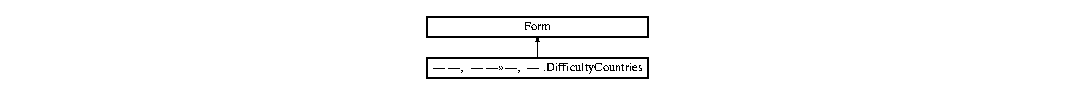
\includegraphics[height=0.830245cm]{class_xD0_x92_xD0_xB8_xD1_x81_xD0_xB5_xD0_xBB_xD0_xB8_xD1_x86_xD0_xB0_1_1_difficulty_countries}
\end{center}
\end{figure}
\subsection*{Открытые члены}
\begin{DoxyCompactItemize}
\item 
\hyperlink{class_xD0_x92_xD0_xB8_xD1_x81_xD0_xB5_xD0_xBB_xD0_xB8_xD1_x86_xD0_xB0_1_1_difficulty_countries_addbad0f815d9ec8edf66c921cc8e9a09}{Difficulty\+Countries} ()
\begin{DoxyCompactList}\small\item\em Метод инициализации \end{DoxyCompactList}\end{DoxyCompactItemize}
\subsection*{Защищенные члены}
\begin{DoxyCompactItemize}
\item 
override void \hyperlink{class_xD0_x92_xD0_xB8_xD1_x81_xD0_xB5_xD0_xBB_xD0_xB8_xD1_x86_xD0_xB0_1_1_difficulty_countries_a010ca1e5b4c957f505030083c2595eb7}{Dispose} (bool disposing)
\begin{DoxyCompactList}\small\item\em Clean up any resources being used. \end{DoxyCompactList}\end{DoxyCompactItemize}


\subsection{Подробное описание}
Класс \hyperlink{class_xD0_x92_xD0_xB8_xD1_x81_xD0_xB5_xD0_xBB_xD0_xB8_xD1_x86_xD0_xB0_1_1_difficulty_countries}{Difficulty\+Countries}. 

Основной и единственный класс, отвечающий за окно выбора уровней сложности для категории стран 

\subsection{Конструктор(ы)}
\hypertarget{class_xD0_x92_xD0_xB8_xD1_x81_xD0_xB5_xD0_xBB_xD0_xB8_xD1_x86_xD0_xB0_1_1_difficulty_countries_addbad0f815d9ec8edf66c921cc8e9a09}{\index{Виселица\+::\+Difficulty\+Countries@{Виселица\+::\+Difficulty\+Countries}!Difficulty\+Countries@{Difficulty\+Countries}}
\index{Difficulty\+Countries@{Difficulty\+Countries}!Виселица\+::\+Difficulty\+Countries@{Виселица\+::\+Difficulty\+Countries}}
\subsubsection[{Difficulty\+Countries}]{\setlength{\rightskip}{0pt plus 5cm}Виселица.\+Difficulty\+Countries.\+Difficulty\+Countries (
\begin{DoxyParamCaption}
{}
\end{DoxyParamCaption}
)\hspace{0.3cm}{\ttfamily [inline]}}}\label{class_xD0_x92_xD0_xB8_xD1_x81_xD0_xB5_xD0_xBB_xD0_xB8_xD1_x86_xD0_xB0_1_1_difficulty_countries_addbad0f815d9ec8edf66c921cc8e9a09}


Метод инициализации 

Инициализация всех компонентов окна Сложность страны 

\subsection{Методы}
\hypertarget{class_xD0_x92_xD0_xB8_xD1_x81_xD0_xB5_xD0_xBB_xD0_xB8_xD1_x86_xD0_xB0_1_1_difficulty_countries_a010ca1e5b4c957f505030083c2595eb7}{\index{Виселица\+::\+Difficulty\+Countries@{Виселица\+::\+Difficulty\+Countries}!Dispose@{Dispose}}
\index{Dispose@{Dispose}!Виселица\+::\+Difficulty\+Countries@{Виселица\+::\+Difficulty\+Countries}}
\subsubsection[{Dispose}]{\setlength{\rightskip}{0pt plus 5cm}override void Виселица.\+Difficulty\+Countries.\+Dispose (
\begin{DoxyParamCaption}
\item[{bool}]{disposing}
\end{DoxyParamCaption}
)\hspace{0.3cm}{\ttfamily [inline]}, {\ttfamily [protected]}}}\label{class_xD0_x92_xD0_xB8_xD1_x81_xD0_xB5_xD0_xBB_xD0_xB8_xD1_x86_xD0_xB0_1_1_difficulty_countries_a010ca1e5b4c957f505030083c2595eb7}


Clean up any resources being used. 


\begin{DoxyParams}{Аргументы}
{\em disposing} & true if managed resources should be disposed; otherwise, false.\\
\hline
\end{DoxyParams}


Объявления и описания членов классов находятся в файлах\+:\begin{DoxyCompactItemize}
\item 
Виселица/Виселица/\hyperlink{_difficulty_countries_8cs}{Difficulty\+Countries.\+cs}\item 
Виселица/Виселица/Difficulty\+Countries.\+Designer.\+cs\end{DoxyCompactItemize}

\hypertarget{class_xD0_x92_xD0_xB8_xD1_x81_xD0_xB5_xD0_xBB_xD0_xB8_xD1_x86_xD0_xB0_1_1_game_average_animals}{\section{Класс Виселица.\+Game\+Average\+Animals}
\label{class_xD0_x92_xD0_xB8_xD1_x81_xD0_xB5_xD0_xBB_xD0_xB8_xD1_x86_xD0_xB0_1_1_game_average_animals}\index{Виселица.\+Game\+Average\+Animals@{Виселица.\+Game\+Average\+Animals}}
}


Класс \hyperlink{class_xD0_x92_xD0_xB8_xD1_x81_xD0_xB5_xD0_xBB_xD0_xB8_xD1_x86_xD0_xB0_1_1_game_average_animals}{Game\+Average\+Animals}.  


Граф наследования\+:Виселица.\+Game\+Average\+Animals\+:\begin{figure}[H]
\begin{center}
\leavevmode

\includegraphics[height=0.817518cm]{class_xD0_x92_xD0_xB8_xD1_x81_xD0_xB5_xD0_xBB_xD0_xB8_xD1_x86_xD0_xB0_1_1_game_average_animals}
\end{center}
\end{figure}
\subsection*{Открытые члены}
\begin{DoxyCompactItemize}
\item 
\hyperlink{class_xD0_x92_xD0_xB8_xD1_x81_xD0_xB5_xD0_xBB_xD0_xB8_xD1_x86_xD0_xB0_1_1_game_average_animals_a6520daaaf168e705f0c21c47faee4e97}{Game\+Average\+Animals} ()
\begin{DoxyCompactList}\small\item\em Метод инициализации \end{DoxyCompactList}\end{DoxyCompactItemize}
\subsection*{Защищенные члены}
\begin{DoxyCompactItemize}
\item 
override void \hyperlink{class_xD0_x92_xD0_xB8_xD1_x81_xD0_xB5_xD0_xBB_xD0_xB8_xD1_x86_xD0_xB0_1_1_game_average_animals_aff15e530827ffb61aa3edb7f0db2f11d}{Dispose} (bool disposing)
\begin{DoxyCompactList}\small\item\em Clean up any resources being used. \end{DoxyCompactList}\end{DoxyCompactItemize}


\subsection{Подробное описание}
Класс \hyperlink{class_xD0_x92_xD0_xB8_xD1_x81_xD0_xB5_xD0_xBB_xD0_xB8_xD1_x86_xD0_xB0_1_1_game_average_animals}{Game\+Average\+Animals}. 

Основной и единственный класс, отвечающий за окно игрового поля для среднего уровня категории животных 

\subsection{Конструктор(ы)}
\hypertarget{class_xD0_x92_xD0_xB8_xD1_x81_xD0_xB5_xD0_xBB_xD0_xB8_xD1_x86_xD0_xB0_1_1_game_average_animals_a6520daaaf168e705f0c21c47faee4e97}{\index{Виселица\+::\+Game\+Average\+Animals@{Виселица\+::\+Game\+Average\+Animals}!Game\+Average\+Animals@{Game\+Average\+Animals}}
\index{Game\+Average\+Animals@{Game\+Average\+Animals}!Виселица\+::\+Game\+Average\+Animals@{Виселица\+::\+Game\+Average\+Animals}}
\subsubsection[{Game\+Average\+Animals}]{\setlength{\rightskip}{0pt plus 5cm}Виселица.\+Game\+Average\+Animals.\+Game\+Average\+Animals (
\begin{DoxyParamCaption}
{}
\end{DoxyParamCaption}
)\hspace{0.3cm}{\ttfamily [inline]}}}\label{class_xD0_x92_xD0_xB8_xD1_x81_xD0_xB5_xD0_xBB_xD0_xB8_xD1_x86_xD0_xB0_1_1_game_average_animals_a6520daaaf168e705f0c21c47faee4e97}


Метод инициализации 

Инициализация всех компонентов окна Игровое поле среднего уровня категории животных 

\subsection{Методы}
\hypertarget{class_xD0_x92_xD0_xB8_xD1_x81_xD0_xB5_xD0_xBB_xD0_xB8_xD1_x86_xD0_xB0_1_1_game_average_animals_aff15e530827ffb61aa3edb7f0db2f11d}{\index{Виселица\+::\+Game\+Average\+Animals@{Виселица\+::\+Game\+Average\+Animals}!Dispose@{Dispose}}
\index{Dispose@{Dispose}!Виселица\+::\+Game\+Average\+Animals@{Виселица\+::\+Game\+Average\+Animals}}
\subsubsection[{Dispose}]{\setlength{\rightskip}{0pt plus 5cm}override void Виселица.\+Game\+Average\+Animals.\+Dispose (
\begin{DoxyParamCaption}
\item[{bool}]{disposing}
\end{DoxyParamCaption}
)\hspace{0.3cm}{\ttfamily [inline]}, {\ttfamily [protected]}}}\label{class_xD0_x92_xD0_xB8_xD1_x81_xD0_xB5_xD0_xBB_xD0_xB8_xD1_x86_xD0_xB0_1_1_game_average_animals_aff15e530827ffb61aa3edb7f0db2f11d}


Clean up any resources being used. 


\begin{DoxyParams}{Аргументы}
{\em disposing} & true if managed resources should be disposed; otherwise, false.\\
\hline
\end{DoxyParams}


Объявления и описания членов классов находятся в файлах\+:\begin{DoxyCompactItemize}
\item 
Виселица/Виселица/\hyperlink{_game_average_animals_8cs}{Game\+Average\+Animals.\+cs}\item 
Виселица/Виселица/Game\+Average\+Animals.\+Designer.\+cs\end{DoxyCompactItemize}

\hypertarget{class_xD0_x92_xD0_xB8_xD1_x81_xD0_xB5_xD0_xBB_xD0_xB8_xD1_x86_xD0_xB0_1_1_game_average_cities}{\section{Класс Виселица.\+Game\+Average\+Cities}
\label{class_xD0_x92_xD0_xB8_xD1_x81_xD0_xB5_xD0_xBB_xD0_xB8_xD1_x86_xD0_xB0_1_1_game_average_cities}\index{Виселица.\+Game\+Average\+Cities@{Виселица.\+Game\+Average\+Cities}}
}


Класс \hyperlink{class_xD0_x92_xD0_xB8_xD1_x81_xD0_xB5_xD0_xBB_xD0_xB8_xD1_x86_xD0_xB0_1_1_game_average_cities}{Game\+Average\+Cities}.  


Граф наследования\+:Виселица.\+Game\+Average\+Cities\+:\begin{figure}[H]
\begin{center}
\leavevmode

\includegraphics[height=0.825350cm]{class_xD0_x92_xD0_xB8_xD1_x81_xD0_xB5_xD0_xBB_xD0_xB8_xD1_x86_xD0_xB0_1_1_game_average_cities}
\end{center}
\end{figure}
\subsection*{Открытые члены}
\begin{DoxyCompactItemize}
\item 
\hyperlink{class_xD0_x92_xD0_xB8_xD1_x81_xD0_xB5_xD0_xBB_xD0_xB8_xD1_x86_xD0_xB0_1_1_game_average_cities_a9d5c6af66340f064859d5b3c6348658b}{Game\+Average\+Cities} ()
\begin{DoxyCompactList}\small\item\em Метод инициализации \end{DoxyCompactList}\end{DoxyCompactItemize}
\subsection*{Защищенные члены}
\begin{DoxyCompactItemize}
\item 
override void \hyperlink{class_xD0_x92_xD0_xB8_xD1_x81_xD0_xB5_xD0_xBB_xD0_xB8_xD1_x86_xD0_xB0_1_1_game_average_cities_a2964196efec7bffeac3fa474af0799a5}{Dispose} (bool disposing)
\begin{DoxyCompactList}\small\item\em Clean up any resources being used. \end{DoxyCompactList}\end{DoxyCompactItemize}


\subsection{Подробное описание}
Класс \hyperlink{class_xD0_x92_xD0_xB8_xD1_x81_xD0_xB5_xD0_xBB_xD0_xB8_xD1_x86_xD0_xB0_1_1_game_average_cities}{Game\+Average\+Cities}. 

Основной и единственный класс, отвечающий за окно игрового поля для среднего уровня категории городов 

\subsection{Конструктор(ы)}
\hypertarget{class_xD0_x92_xD0_xB8_xD1_x81_xD0_xB5_xD0_xBB_xD0_xB8_xD1_x86_xD0_xB0_1_1_game_average_cities_a9d5c6af66340f064859d5b3c6348658b}{\index{Виселица\+::\+Game\+Average\+Cities@{Виселица\+::\+Game\+Average\+Cities}!Game\+Average\+Cities@{Game\+Average\+Cities}}
\index{Game\+Average\+Cities@{Game\+Average\+Cities}!Виселица\+::\+Game\+Average\+Cities@{Виселица\+::\+Game\+Average\+Cities}}
\subsubsection[{Game\+Average\+Cities}]{\setlength{\rightskip}{0pt plus 5cm}Виселица.\+Game\+Average\+Cities.\+Game\+Average\+Cities (
\begin{DoxyParamCaption}
{}
\end{DoxyParamCaption}
)\hspace{0.3cm}{\ttfamily [inline]}}}\label{class_xD0_x92_xD0_xB8_xD1_x81_xD0_xB5_xD0_xBB_xD0_xB8_xD1_x86_xD0_xB0_1_1_game_average_cities_a9d5c6af66340f064859d5b3c6348658b}


Метод инициализации 

Инициализация всех компонентов окна Игровое поле среднего уровня категории городов 

\subsection{Методы}
\hypertarget{class_xD0_x92_xD0_xB8_xD1_x81_xD0_xB5_xD0_xBB_xD0_xB8_xD1_x86_xD0_xB0_1_1_game_average_cities_a2964196efec7bffeac3fa474af0799a5}{\index{Виселица\+::\+Game\+Average\+Cities@{Виселица\+::\+Game\+Average\+Cities}!Dispose@{Dispose}}
\index{Dispose@{Dispose}!Виселица\+::\+Game\+Average\+Cities@{Виселица\+::\+Game\+Average\+Cities}}
\subsubsection[{Dispose}]{\setlength{\rightskip}{0pt plus 5cm}override void Виселица.\+Game\+Average\+Cities.\+Dispose (
\begin{DoxyParamCaption}
\item[{bool}]{disposing}
\end{DoxyParamCaption}
)\hspace{0.3cm}{\ttfamily [inline]}, {\ttfamily [protected]}}}\label{class_xD0_x92_xD0_xB8_xD1_x81_xD0_xB5_xD0_xBB_xD0_xB8_xD1_x86_xD0_xB0_1_1_game_average_cities_a2964196efec7bffeac3fa474af0799a5}


Clean up any resources being used. 


\begin{DoxyParams}{Аргументы}
{\em disposing} & true if managed resources should be disposed; otherwise, false.\\
\hline
\end{DoxyParams}


Объявления и описания членов классов находятся в файлах\+:\begin{DoxyCompactItemize}
\item 
Виселица/Виселица/\hyperlink{_game_average_cities_8cs}{Game\+Average\+Cities.\+cs}\item 
Виселица/Виселица/Game\+Average\+Cities.\+Designer.\+cs\end{DoxyCompactItemize}

\hypertarget{class_xD0_x92_xD0_xB8_xD1_x81_xD0_xB5_xD0_xBB_xD0_xB8_xD1_x86_xD0_xB0_1_1_game_average_countries}{\section{Класс Виселица.\+Game\+Average\+Countries}
\label{class_xD0_x92_xD0_xB8_xD1_x81_xD0_xB5_xD0_xBB_xD0_xB8_xD1_x86_xD0_xB0_1_1_game_average_countries}\index{Виселица.\+Game\+Average\+Countries@{Виселица.\+Game\+Average\+Countries}}
}


Класс \hyperlink{class_xD0_x92_xD0_xB8_xD1_x81_xD0_xB5_xD0_xBB_xD0_xB8_xD1_x86_xD0_xB0_1_1_game_average_countries}{Game\+Average\+Countries}.  


Граф наследования\+:Виселица.\+Game\+Average\+Countries\+:\begin{figure}[H]
\begin{center}
\leavevmode

\includegraphics[height=0.811594cm]{class_xD0_x92_xD0_xB8_xD1_x81_xD0_xB5_xD0_xBB_xD0_xB8_xD1_x86_xD0_xB0_1_1_game_average_countries}
\end{center}
\end{figure}
\subsection*{Открытые члены}
\begin{DoxyCompactItemize}
\item 
\hyperlink{class_xD0_x92_xD0_xB8_xD1_x81_xD0_xB5_xD0_xBB_xD0_xB8_xD1_x86_xD0_xB0_1_1_game_average_countries_a686c439b5f74cee1da56f04ecbd507ea}{Game\+Average\+Countries} ()
\begin{DoxyCompactList}\small\item\em Метод инициализации \end{DoxyCompactList}\end{DoxyCompactItemize}
\subsection*{Защищенные члены}
\begin{DoxyCompactItemize}
\item 
override void \hyperlink{class_xD0_x92_xD0_xB8_xD1_x81_xD0_xB5_xD0_xBB_xD0_xB8_xD1_x86_xD0_xB0_1_1_game_average_countries_a5cbc95f48e9310b5b91ac2585a11467a}{Dispose} (bool disposing)
\begin{DoxyCompactList}\small\item\em Clean up any resources being used. \end{DoxyCompactList}\end{DoxyCompactItemize}


\subsection{Подробное описание}
Класс \hyperlink{class_xD0_x92_xD0_xB8_xD1_x81_xD0_xB5_xD0_xBB_xD0_xB8_xD1_x86_xD0_xB0_1_1_game_average_countries}{Game\+Average\+Countries}. 

Основной и единственный класс, отвечающий за окно игрового поля для среднего уровня категории стран 

\subsection{Конструктор(ы)}
\hypertarget{class_xD0_x92_xD0_xB8_xD1_x81_xD0_xB5_xD0_xBB_xD0_xB8_xD1_x86_xD0_xB0_1_1_game_average_countries_a686c439b5f74cee1da56f04ecbd507ea}{\index{Виселица\+::\+Game\+Average\+Countries@{Виселица\+::\+Game\+Average\+Countries}!Game\+Average\+Countries@{Game\+Average\+Countries}}
\index{Game\+Average\+Countries@{Game\+Average\+Countries}!Виселица\+::\+Game\+Average\+Countries@{Виселица\+::\+Game\+Average\+Countries}}
\subsubsection[{Game\+Average\+Countries}]{\setlength{\rightskip}{0pt plus 5cm}Виселица.\+Game\+Average\+Countries.\+Game\+Average\+Countries (
\begin{DoxyParamCaption}
{}
\end{DoxyParamCaption}
)\hspace{0.3cm}{\ttfamily [inline]}}}\label{class_xD0_x92_xD0_xB8_xD1_x81_xD0_xB5_xD0_xBB_xD0_xB8_xD1_x86_xD0_xB0_1_1_game_average_countries_a686c439b5f74cee1da56f04ecbd507ea}


Метод инициализации 

Инициализация всех компонентов окна Игровое поле среднего уровня категории стран 

\subsection{Методы}
\hypertarget{class_xD0_x92_xD0_xB8_xD1_x81_xD0_xB5_xD0_xBB_xD0_xB8_xD1_x86_xD0_xB0_1_1_game_average_countries_a5cbc95f48e9310b5b91ac2585a11467a}{\index{Виселица\+::\+Game\+Average\+Countries@{Виселица\+::\+Game\+Average\+Countries}!Dispose@{Dispose}}
\index{Dispose@{Dispose}!Виселица\+::\+Game\+Average\+Countries@{Виселица\+::\+Game\+Average\+Countries}}
\subsubsection[{Dispose}]{\setlength{\rightskip}{0pt plus 5cm}override void Виселица.\+Game\+Average\+Countries.\+Dispose (
\begin{DoxyParamCaption}
\item[{bool}]{disposing}
\end{DoxyParamCaption}
)\hspace{0.3cm}{\ttfamily [inline]}, {\ttfamily [protected]}}}\label{class_xD0_x92_xD0_xB8_xD1_x81_xD0_xB5_xD0_xBB_xD0_xB8_xD1_x86_xD0_xB0_1_1_game_average_countries_a5cbc95f48e9310b5b91ac2585a11467a}


Clean up any resources being used. 


\begin{DoxyParams}{Аргументы}
{\em disposing} & true if managed resources should be disposed; otherwise, false.\\
\hline
\end{DoxyParams}


Объявления и описания членов классов находятся в файлах\+:\begin{DoxyCompactItemize}
\item 
Виселица/Виселица/\hyperlink{_game_average_countries_8cs}{Game\+Average\+Countries.\+cs}\item 
Виселица/Виселица/Game\+Average\+Countries.\+Designer.\+cs\end{DoxyCompactItemize}

\hypertarget{class_xD0_x92_xD0_xB8_xD1_x81_xD0_xB5_xD0_xBB_xD0_xB8_xD1_x86_xD0_xB0_1_1_game_difficult_animals}{\section{Класс Виселица.\+Game\+Difficult\+Animals}
\label{class_xD0_x92_xD0_xB8_xD1_x81_xD0_xB5_xD0_xBB_xD0_xB8_xD1_x86_xD0_xB0_1_1_game_difficult_animals}\index{Виселица.\+Game\+Difficult\+Animals@{Виселица.\+Game\+Difficult\+Animals}}
}


Класс \hyperlink{class_xD0_x92_xD0_xB8_xD1_x81_xD0_xB5_xD0_xBB_xD0_xB8_xD1_x86_xD0_xB0_1_1_game_difficult_animals}{Game\+Difficult\+Animals}.  


Граф наследования\+:Виселица.\+Game\+Difficult\+Animals\+:\begin{figure}[H]
\begin{center}
\leavevmode
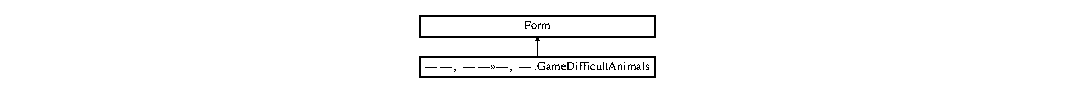
\includegraphics[height=0.821114cm]{class_xD0_x92_xD0_xB8_xD1_x81_xD0_xB5_xD0_xBB_xD0_xB8_xD1_x86_xD0_xB0_1_1_game_difficult_animals}
\end{center}
\end{figure}
\subsection*{Открытые члены}
\begin{DoxyCompactItemize}
\item 
\hyperlink{class_xD0_x92_xD0_xB8_xD1_x81_xD0_xB5_xD0_xBB_xD0_xB8_xD1_x86_xD0_xB0_1_1_game_difficult_animals_a49213804e9bc6c825cf719237718bb48}{Game\+Difficult\+Animals} ()
\begin{DoxyCompactList}\small\item\em Метод инициализации \end{DoxyCompactList}\end{DoxyCompactItemize}
\subsection*{Защищенные члены}
\begin{DoxyCompactItemize}
\item 
override void \hyperlink{class_xD0_x92_xD0_xB8_xD1_x81_xD0_xB5_xD0_xBB_xD0_xB8_xD1_x86_xD0_xB0_1_1_game_difficult_animals_af05de0debfe8cfe88b78d0c91efe2aba}{Dispose} (bool disposing)
\begin{DoxyCompactList}\small\item\em Clean up any resources being used. \end{DoxyCompactList}\end{DoxyCompactItemize}


\subsection{Подробное описание}
Класс \hyperlink{class_xD0_x92_xD0_xB8_xD1_x81_xD0_xB5_xD0_xBB_xD0_xB8_xD1_x86_xD0_xB0_1_1_game_difficult_animals}{Game\+Difficult\+Animals}. 

Основной и единственный класс, отвечающий за окно игрового поля для сложного уровня категории животных 

\subsection{Конструктор(ы)}
\hypertarget{class_xD0_x92_xD0_xB8_xD1_x81_xD0_xB5_xD0_xBB_xD0_xB8_xD1_x86_xD0_xB0_1_1_game_difficult_animals_a49213804e9bc6c825cf719237718bb48}{\index{Виселица\+::\+Game\+Difficult\+Animals@{Виселица\+::\+Game\+Difficult\+Animals}!Game\+Difficult\+Animals@{Game\+Difficult\+Animals}}
\index{Game\+Difficult\+Animals@{Game\+Difficult\+Animals}!Виселица\+::\+Game\+Difficult\+Animals@{Виселица\+::\+Game\+Difficult\+Animals}}
\subsubsection[{Game\+Difficult\+Animals}]{\setlength{\rightskip}{0pt plus 5cm}Виселица.\+Game\+Difficult\+Animals.\+Game\+Difficult\+Animals (
\begin{DoxyParamCaption}
{}
\end{DoxyParamCaption}
)\hspace{0.3cm}{\ttfamily [inline]}}}\label{class_xD0_x92_xD0_xB8_xD1_x81_xD0_xB5_xD0_xBB_xD0_xB8_xD1_x86_xD0_xB0_1_1_game_difficult_animals_a49213804e9bc6c825cf719237718bb48}


Метод инициализации 

Инициализация всех компонентов окна Игровое поле сложного уровня категории животных 

\subsection{Методы}
\hypertarget{class_xD0_x92_xD0_xB8_xD1_x81_xD0_xB5_xD0_xBB_xD0_xB8_xD1_x86_xD0_xB0_1_1_game_difficult_animals_af05de0debfe8cfe88b78d0c91efe2aba}{\index{Виселица\+::\+Game\+Difficult\+Animals@{Виселица\+::\+Game\+Difficult\+Animals}!Dispose@{Dispose}}
\index{Dispose@{Dispose}!Виселица\+::\+Game\+Difficult\+Animals@{Виселица\+::\+Game\+Difficult\+Animals}}
\subsubsection[{Dispose}]{\setlength{\rightskip}{0pt plus 5cm}override void Виселица.\+Game\+Difficult\+Animals.\+Dispose (
\begin{DoxyParamCaption}
\item[{bool}]{disposing}
\end{DoxyParamCaption}
)\hspace{0.3cm}{\ttfamily [inline]}, {\ttfamily [protected]}}}\label{class_xD0_x92_xD0_xB8_xD1_x81_xD0_xB5_xD0_xBB_xD0_xB8_xD1_x86_xD0_xB0_1_1_game_difficult_animals_af05de0debfe8cfe88b78d0c91efe2aba}


Clean up any resources being used. 


\begin{DoxyParams}{Аргументы}
{\em disposing} & true if managed resources should be disposed; otherwise, false.\\
\hline
\end{DoxyParams}


Объявления и описания членов классов находятся в файлах\+:\begin{DoxyCompactItemize}
\item 
Виселица/Виселица/\hyperlink{_game_difficult_animals_8cs}{Game\+Difficult\+Animals.\+cs}\item 
Виселица/Виселица/Game\+Difficult\+Animals.\+Designer.\+cs\end{DoxyCompactItemize}

\hypertarget{class_xD0_x92_xD0_xB8_xD1_x81_xD0_xB5_xD0_xBB_xD0_xB8_xD1_x86_xD0_xB0_1_1_game_difficult_cities}{\section{Класс Виселица.\+Game\+Difficult\+Cities}
\label{class_xD0_x92_xD0_xB8_xD1_x81_xD0_xB5_xD0_xBB_xD0_xB8_xD1_x86_xD0_xB0_1_1_game_difficult_cities}\index{Виселица.\+Game\+Difficult\+Cities@{Виселица.\+Game\+Difficult\+Cities}}
}


Класс \hyperlink{class_xD0_x92_xD0_xB8_xD1_x81_xD0_xB5_xD0_xBB_xD0_xB8_xD1_x86_xD0_xB0_1_1_game_difficult_cities}{Game\+Difficult\+Cities}.  


Граф наследования\+:Виселица.\+Game\+Difficult\+Cities\+:\begin{figure}[H]
\begin{center}
\leavevmode
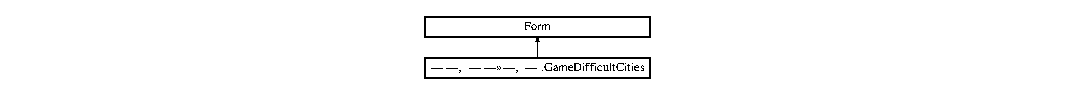
\includegraphics[height=0.829015cm]{class_xD0_x92_xD0_xB8_xD1_x81_xD0_xB5_xD0_xBB_xD0_xB8_xD1_x86_xD0_xB0_1_1_game_difficult_cities}
\end{center}
\end{figure}
\subsection*{Открытые члены}
\begin{DoxyCompactItemize}
\item 
\hyperlink{class_xD0_x92_xD0_xB8_xD1_x81_xD0_xB5_xD0_xBB_xD0_xB8_xD1_x86_xD0_xB0_1_1_game_difficult_cities_ac44fc6d861eac3a3c990fcf2fd0de7e2}{Game\+Difficult\+Cities} ()
\begin{DoxyCompactList}\small\item\em Метод инициализации \end{DoxyCompactList}\end{DoxyCompactItemize}
\subsection*{Защищенные члены}
\begin{DoxyCompactItemize}
\item 
override void \hyperlink{class_xD0_x92_xD0_xB8_xD1_x81_xD0_xB5_xD0_xBB_xD0_xB8_xD1_x86_xD0_xB0_1_1_game_difficult_cities_a45567bf0f1366f555d84b7b21baf91c6}{Dispose} (bool disposing)
\begin{DoxyCompactList}\small\item\em Clean up any resources being used. \end{DoxyCompactList}\end{DoxyCompactItemize}


\subsection{Подробное описание}
Класс \hyperlink{class_xD0_x92_xD0_xB8_xD1_x81_xD0_xB5_xD0_xBB_xD0_xB8_xD1_x86_xD0_xB0_1_1_game_difficult_cities}{Game\+Difficult\+Cities}. 

Основной и единственный класс, отвечающий за окно игрового поля для сложного уровня категории городов 

\subsection{Конструктор(ы)}
\hypertarget{class_xD0_x92_xD0_xB8_xD1_x81_xD0_xB5_xD0_xBB_xD0_xB8_xD1_x86_xD0_xB0_1_1_game_difficult_cities_ac44fc6d861eac3a3c990fcf2fd0de7e2}{\index{Виселица\+::\+Game\+Difficult\+Cities@{Виселица\+::\+Game\+Difficult\+Cities}!Game\+Difficult\+Cities@{Game\+Difficult\+Cities}}
\index{Game\+Difficult\+Cities@{Game\+Difficult\+Cities}!Виселица\+::\+Game\+Difficult\+Cities@{Виселица\+::\+Game\+Difficult\+Cities}}
\subsubsection[{Game\+Difficult\+Cities}]{\setlength{\rightskip}{0pt plus 5cm}Виселица.\+Game\+Difficult\+Cities.\+Game\+Difficult\+Cities (
\begin{DoxyParamCaption}
{}
\end{DoxyParamCaption}
)\hspace{0.3cm}{\ttfamily [inline]}}}\label{class_xD0_x92_xD0_xB8_xD1_x81_xD0_xB5_xD0_xBB_xD0_xB8_xD1_x86_xD0_xB0_1_1_game_difficult_cities_ac44fc6d861eac3a3c990fcf2fd0de7e2}


Метод инициализации 

Инициализация всех компонентов окна Игровое поле сложного уровня категории городов 

\subsection{Методы}
\hypertarget{class_xD0_x92_xD0_xB8_xD1_x81_xD0_xB5_xD0_xBB_xD0_xB8_xD1_x86_xD0_xB0_1_1_game_difficult_cities_a45567bf0f1366f555d84b7b21baf91c6}{\index{Виселица\+::\+Game\+Difficult\+Cities@{Виселица\+::\+Game\+Difficult\+Cities}!Dispose@{Dispose}}
\index{Dispose@{Dispose}!Виселица\+::\+Game\+Difficult\+Cities@{Виселица\+::\+Game\+Difficult\+Cities}}
\subsubsection[{Dispose}]{\setlength{\rightskip}{0pt plus 5cm}override void Виселица.\+Game\+Difficult\+Cities.\+Dispose (
\begin{DoxyParamCaption}
\item[{bool}]{disposing}
\end{DoxyParamCaption}
)\hspace{0.3cm}{\ttfamily [inline]}, {\ttfamily [protected]}}}\label{class_xD0_x92_xD0_xB8_xD1_x81_xD0_xB5_xD0_xBB_xD0_xB8_xD1_x86_xD0_xB0_1_1_game_difficult_cities_a45567bf0f1366f555d84b7b21baf91c6}


Clean up any resources being used. 


\begin{DoxyParams}{Аргументы}
{\em disposing} & true if managed resources should be disposed; otherwise, false.\\
\hline
\end{DoxyParams}


Объявления и описания членов классов находятся в файлах\+:\begin{DoxyCompactItemize}
\item 
Виселица/Виселица/\hyperlink{_game_difficult_cities_8cs}{Game\+Difficult\+Cities.\+cs}\item 
Виселица/Виселица/Game\+Difficult\+Cities.\+Designer.\+cs\end{DoxyCompactItemize}

\hypertarget{class_xD0_x92_xD0_xB8_xD1_x81_xD0_xB5_xD0_xBB_xD0_xB8_xD1_x86_xD0_xB0_1_1_game_difficult_countries}{\section{Класс Виселица.\+Game\+Difficult\+Countries}
\label{class_xD0_x92_xD0_xB8_xD1_x81_xD0_xB5_xD0_xBB_xD0_xB8_xD1_x86_xD0_xB0_1_1_game_difficult_countries}\index{Виселица.\+Game\+Difficult\+Countries@{Виселица.\+Game\+Difficult\+Countries}}
}


Класс \hyperlink{class_xD0_x92_xD0_xB8_xD1_x81_xD0_xB5_xD0_xBB_xD0_xB8_xD1_x86_xD0_xB0_1_1_game_difficult_countries}{Game\+Difficult\+Countries}.  


Граф наследования\+:Виселица.\+Game\+Difficult\+Countries\+:\begin{figure}[H]
\begin{center}
\leavevmode

\includegraphics[height=0.815138cm]{class_xD0_x92_xD0_xB8_xD1_x81_xD0_xB5_xD0_xBB_xD0_xB8_xD1_x86_xD0_xB0_1_1_game_difficult_countries}
\end{center}
\end{figure}
\subsection*{Открытые члены}
\begin{DoxyCompactItemize}
\item 
\hyperlink{class_xD0_x92_xD0_xB8_xD1_x81_xD0_xB5_xD0_xBB_xD0_xB8_xD1_x86_xD0_xB0_1_1_game_difficult_countries_a387325ece898d55c197ba03da390a47d}{Game\+Difficult\+Countries} ()
\begin{DoxyCompactList}\small\item\em Метод инициализации \end{DoxyCompactList}\end{DoxyCompactItemize}
\subsection*{Защищенные члены}
\begin{DoxyCompactItemize}
\item 
override void \hyperlink{class_xD0_x92_xD0_xB8_xD1_x81_xD0_xB5_xD0_xBB_xD0_xB8_xD1_x86_xD0_xB0_1_1_game_difficult_countries_af7eea88e8a69c00ceab22485bc504d69}{Dispose} (bool disposing)
\begin{DoxyCompactList}\small\item\em Clean up any resources being used. \end{DoxyCompactList}\end{DoxyCompactItemize}


\subsection{Подробное описание}
Класс \hyperlink{class_xD0_x92_xD0_xB8_xD1_x81_xD0_xB5_xD0_xBB_xD0_xB8_xD1_x86_xD0_xB0_1_1_game_difficult_countries}{Game\+Difficult\+Countries}. 

Основной и единственный класс, отвечающий за окно игрового поля для сложного уровня категории стран 

\subsection{Конструктор(ы)}
\hypertarget{class_xD0_x92_xD0_xB8_xD1_x81_xD0_xB5_xD0_xBB_xD0_xB8_xD1_x86_xD0_xB0_1_1_game_difficult_countries_a387325ece898d55c197ba03da390a47d}{\index{Виселица\+::\+Game\+Difficult\+Countries@{Виселица\+::\+Game\+Difficult\+Countries}!Game\+Difficult\+Countries@{Game\+Difficult\+Countries}}
\index{Game\+Difficult\+Countries@{Game\+Difficult\+Countries}!Виселица\+::\+Game\+Difficult\+Countries@{Виселица\+::\+Game\+Difficult\+Countries}}
\subsubsection[{Game\+Difficult\+Countries}]{\setlength{\rightskip}{0pt plus 5cm}Виселица.\+Game\+Difficult\+Countries.\+Game\+Difficult\+Countries (
\begin{DoxyParamCaption}
{}
\end{DoxyParamCaption}
)\hspace{0.3cm}{\ttfamily [inline]}}}\label{class_xD0_x92_xD0_xB8_xD1_x81_xD0_xB5_xD0_xBB_xD0_xB8_xD1_x86_xD0_xB0_1_1_game_difficult_countries_a387325ece898d55c197ba03da390a47d}


Метод инициализации 

Инициализация всех компонентов окна Игровое поле сложного уровня категории стран 

\subsection{Методы}
\hypertarget{class_xD0_x92_xD0_xB8_xD1_x81_xD0_xB5_xD0_xBB_xD0_xB8_xD1_x86_xD0_xB0_1_1_game_difficult_countries_af7eea88e8a69c00ceab22485bc504d69}{\index{Виселица\+::\+Game\+Difficult\+Countries@{Виселица\+::\+Game\+Difficult\+Countries}!Dispose@{Dispose}}
\index{Dispose@{Dispose}!Виселица\+::\+Game\+Difficult\+Countries@{Виселица\+::\+Game\+Difficult\+Countries}}
\subsubsection[{Dispose}]{\setlength{\rightskip}{0pt plus 5cm}override void Виселица.\+Game\+Difficult\+Countries.\+Dispose (
\begin{DoxyParamCaption}
\item[{bool}]{disposing}
\end{DoxyParamCaption}
)\hspace{0.3cm}{\ttfamily [inline]}, {\ttfamily [protected]}}}\label{class_xD0_x92_xD0_xB8_xD1_x81_xD0_xB5_xD0_xBB_xD0_xB8_xD1_x86_xD0_xB0_1_1_game_difficult_countries_af7eea88e8a69c00ceab22485bc504d69}


Clean up any resources being used. 


\begin{DoxyParams}{Аргументы}
{\em disposing} & true if managed resources should be disposed; otherwise, false.\\
\hline
\end{DoxyParams}


Объявления и описания членов классов находятся в файлах\+:\begin{DoxyCompactItemize}
\item 
Виселица/Виселица/\hyperlink{_game_difficult_countries_8cs}{Game\+Difficult\+Countries.\+cs}\item 
Виселица/Виселица/Game\+Difficult\+Countries.\+Designer.\+cs\end{DoxyCompactItemize}

\hypertarget{class_xD0_x92_xD0_xB8_xD1_x81_xD0_xB5_xD0_xBB_xD0_xB8_xD1_x86_xD0_xB0_1_1_game_light_animals}{\section{Класс Виселица.\+Game\+Light\+Animals}
\label{class_xD0_x92_xD0_xB8_xD1_x81_xD0_xB5_xD0_xBB_xD0_xB8_xD1_x86_xD0_xB0_1_1_game_light_animals}\index{Виселица.\+Game\+Light\+Animals@{Виселица.\+Game\+Light\+Animals}}
}


Класс \hyperlink{class_xD0_x92_xD0_xB8_xD1_x81_xD0_xB5_xD0_xBB_xD0_xB8_xD1_x86_xD0_xB0_1_1_game_light_animals}{Game\+Light\+Animals}.  


Граф наследования\+:Виселица.\+Game\+Light\+Animals\+:\begin{figure}[H]
\begin{center}
\leavevmode

\includegraphics[height=0.830860cm]{class_xD0_x92_xD0_xB8_xD1_x81_xD0_xB5_xD0_xBB_xD0_xB8_xD1_x86_xD0_xB0_1_1_game_light_animals}
\end{center}
\end{figure}
\subsection*{Открытые члены}
\begin{DoxyCompactItemize}
\item 
\hyperlink{class_xD0_x92_xD0_xB8_xD1_x81_xD0_xB5_xD0_xBB_xD0_xB8_xD1_x86_xD0_xB0_1_1_game_light_animals_a1a99aefd2bbf2efaf512a19b501b8595}{Game\+Light\+Animals} ()
\begin{DoxyCompactList}\small\item\em Метод инициализации \end{DoxyCompactList}\end{DoxyCompactItemize}
\subsection*{Защищенные члены}
\begin{DoxyCompactItemize}
\item 
override void \hyperlink{class_xD0_x92_xD0_xB8_xD1_x81_xD0_xB5_xD0_xBB_xD0_xB8_xD1_x86_xD0_xB0_1_1_game_light_animals_a4dcd587a0ab653b506713254151d3abb}{Dispose} (bool disposing)
\begin{DoxyCompactList}\small\item\em Clean up any resources being used. \end{DoxyCompactList}\end{DoxyCompactItemize}


\subsection{Подробное описание}
Класс \hyperlink{class_xD0_x92_xD0_xB8_xD1_x81_xD0_xB5_xD0_xBB_xD0_xB8_xD1_x86_xD0_xB0_1_1_game_light_animals}{Game\+Light\+Animals}. 

Основной и единственный класс, отвечающий за окно игрового поля для лёгкого уровня категории животных 

\subsection{Конструктор(ы)}
\hypertarget{class_xD0_x92_xD0_xB8_xD1_x81_xD0_xB5_xD0_xBB_xD0_xB8_xD1_x86_xD0_xB0_1_1_game_light_animals_a1a99aefd2bbf2efaf512a19b501b8595}{\index{Виселица\+::\+Game\+Light\+Animals@{Виселица\+::\+Game\+Light\+Animals}!Game\+Light\+Animals@{Game\+Light\+Animals}}
\index{Game\+Light\+Animals@{Game\+Light\+Animals}!Виселица\+::\+Game\+Light\+Animals@{Виселица\+::\+Game\+Light\+Animals}}
\subsubsection[{Game\+Light\+Animals}]{\setlength{\rightskip}{0pt plus 5cm}Виселица.\+Game\+Light\+Animals.\+Game\+Light\+Animals (
\begin{DoxyParamCaption}
{}
\end{DoxyParamCaption}
)\hspace{0.3cm}{\ttfamily [inline]}}}\label{class_xD0_x92_xD0_xB8_xD1_x81_xD0_xB5_xD0_xBB_xD0_xB8_xD1_x86_xD0_xB0_1_1_game_light_animals_a1a99aefd2bbf2efaf512a19b501b8595}


Метод инициализации 

Инициализация всех компонентов окна Игровое поле лёгкого уровня категории животных 

\subsection{Методы}
\hypertarget{class_xD0_x92_xD0_xB8_xD1_x81_xD0_xB5_xD0_xBB_xD0_xB8_xD1_x86_xD0_xB0_1_1_game_light_animals_a4dcd587a0ab653b506713254151d3abb}{\index{Виселица\+::\+Game\+Light\+Animals@{Виселица\+::\+Game\+Light\+Animals}!Dispose@{Dispose}}
\index{Dispose@{Dispose}!Виселица\+::\+Game\+Light\+Animals@{Виселица\+::\+Game\+Light\+Animals}}
\subsubsection[{Dispose}]{\setlength{\rightskip}{0pt plus 5cm}override void Виселица.\+Game\+Light\+Animals.\+Dispose (
\begin{DoxyParamCaption}
\item[{bool}]{disposing}
\end{DoxyParamCaption}
)\hspace{0.3cm}{\ttfamily [inline]}, {\ttfamily [protected]}}}\label{class_xD0_x92_xD0_xB8_xD1_x81_xD0_xB5_xD0_xBB_xD0_xB8_xD1_x86_xD0_xB0_1_1_game_light_animals_a4dcd587a0ab653b506713254151d3abb}


Clean up any resources being used. 


\begin{DoxyParams}{Аргументы}
{\em disposing} & true if managed resources should be disposed; otherwise, false.\\
\hline
\end{DoxyParams}


Объявления и описания членов классов находятся в файлах\+:\begin{DoxyCompactItemize}
\item 
Виселица/Виселица/\hyperlink{_game_light_animals_8cs}{Game\+Light\+Animals.\+cs}\item 
Виселица/Виселица/Game\+Light\+Animals.\+Designer.\+cs\end{DoxyCompactItemize}

\hypertarget{class_xD0_x92_xD0_xB8_xD1_x81_xD0_xB5_xD0_xBB_xD0_xB8_xD1_x86_xD0_xB0_1_1_game_light_cities}{\section{Класс Виселица.\+Game\+Light\+Cities}
\label{class_xD0_x92_xD0_xB8_xD1_x81_xD0_xB5_xD0_xBB_xD0_xB8_xD1_x86_xD0_xB0_1_1_game_light_cities}\index{Виселица.\+Game\+Light\+Cities@{Виселица.\+Game\+Light\+Cities}}
}


Класс \hyperlink{class_xD0_x92_xD0_xB8_xD1_x81_xD0_xB5_xD0_xBB_xD0_xB8_xD1_x86_xD0_xB0_1_1_game_light_cities}{Game\+Light\+Cities}.  


Граф наследования\+:Виселица.\+Game\+Light\+Cities\+:\begin{figure}[H]
\begin{center}
\leavevmode
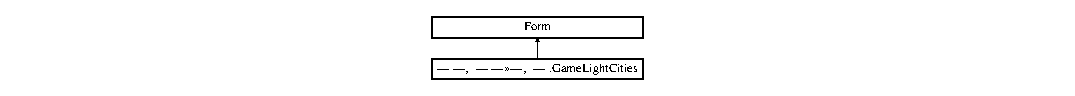
\includegraphics[height=0.838951cm]{class_xD0_x92_xD0_xB8_xD1_x81_xD0_xB5_xD0_xBB_xD0_xB8_xD1_x86_xD0_xB0_1_1_game_light_cities}
\end{center}
\end{figure}
\subsection*{Открытые члены}
\begin{DoxyCompactItemize}
\item 
\hyperlink{class_xD0_x92_xD0_xB8_xD1_x81_xD0_xB5_xD0_xBB_xD0_xB8_xD1_x86_xD0_xB0_1_1_game_light_cities_aa96b7308bf950e95d6a1af8f811dbe4b}{Game\+Light\+Cities} ()
\begin{DoxyCompactList}\small\item\em Метод инициализации \end{DoxyCompactList}\end{DoxyCompactItemize}
\subsection*{Защищенные члены}
\begin{DoxyCompactItemize}
\item 
override void \hyperlink{class_xD0_x92_xD0_xB8_xD1_x81_xD0_xB5_xD0_xBB_xD0_xB8_xD1_x86_xD0_xB0_1_1_game_light_cities_a41cb54fc2a796ceb9f08ed76adce0586}{Dispose} (bool disposing)
\begin{DoxyCompactList}\small\item\em Clean up any resources being used. \end{DoxyCompactList}\end{DoxyCompactItemize}


\subsection{Подробное описание}
Класс \hyperlink{class_xD0_x92_xD0_xB8_xD1_x81_xD0_xB5_xD0_xBB_xD0_xB8_xD1_x86_xD0_xB0_1_1_game_light_cities}{Game\+Light\+Cities}. 

Основной и единственный класс, отвечающий за окно игрового поля для лёгкого уровня категории городов 

\subsection{Конструктор(ы)}
\hypertarget{class_xD0_x92_xD0_xB8_xD1_x81_xD0_xB5_xD0_xBB_xD0_xB8_xD1_x86_xD0_xB0_1_1_game_light_cities_aa96b7308bf950e95d6a1af8f811dbe4b}{\index{Виселица\+::\+Game\+Light\+Cities@{Виселица\+::\+Game\+Light\+Cities}!Game\+Light\+Cities@{Game\+Light\+Cities}}
\index{Game\+Light\+Cities@{Game\+Light\+Cities}!Виселица\+::\+Game\+Light\+Cities@{Виселица\+::\+Game\+Light\+Cities}}
\subsubsection[{Game\+Light\+Cities}]{\setlength{\rightskip}{0pt plus 5cm}Виселица.\+Game\+Light\+Cities.\+Game\+Light\+Cities (
\begin{DoxyParamCaption}
{}
\end{DoxyParamCaption}
)\hspace{0.3cm}{\ttfamily [inline]}}}\label{class_xD0_x92_xD0_xB8_xD1_x81_xD0_xB5_xD0_xBB_xD0_xB8_xD1_x86_xD0_xB0_1_1_game_light_cities_aa96b7308bf950e95d6a1af8f811dbe4b}


Метод инициализации 

Инициализация всех компонентов окна Игровое поле лёгкого уровня категории животных 

\subsection{Методы}
\hypertarget{class_xD0_x92_xD0_xB8_xD1_x81_xD0_xB5_xD0_xBB_xD0_xB8_xD1_x86_xD0_xB0_1_1_game_light_cities_a41cb54fc2a796ceb9f08ed76adce0586}{\index{Виселица\+::\+Game\+Light\+Cities@{Виселица\+::\+Game\+Light\+Cities}!Dispose@{Dispose}}
\index{Dispose@{Dispose}!Виселица\+::\+Game\+Light\+Cities@{Виселица\+::\+Game\+Light\+Cities}}
\subsubsection[{Dispose}]{\setlength{\rightskip}{0pt plus 5cm}override void Виселица.\+Game\+Light\+Cities.\+Dispose (
\begin{DoxyParamCaption}
\item[{bool}]{disposing}
\end{DoxyParamCaption}
)\hspace{0.3cm}{\ttfamily [inline]}, {\ttfamily [protected]}}}\label{class_xD0_x92_xD0_xB8_xD1_x81_xD0_xB5_xD0_xBB_xD0_xB8_xD1_x86_xD0_xB0_1_1_game_light_cities_a41cb54fc2a796ceb9f08ed76adce0586}


Clean up any resources being used. 


\begin{DoxyParams}{Аргументы}
{\em disposing} & true if managed resources should be disposed; otherwise, false.\\
\hline
\end{DoxyParams}


Объявления и описания членов классов находятся в файлах\+:\begin{DoxyCompactItemize}
\item 
Виселица/Виселица/\hyperlink{_game_light_cities_8cs}{Game\+Light\+Cities.\+cs}\item 
Виселица/Виселица/Game\+Light\+Cities.\+Designer.\+cs\end{DoxyCompactItemize}

\hypertarget{class_xD0_x92_xD0_xB8_xD1_x81_xD0_xB5_xD0_xBB_xD0_xB8_xD1_x86_xD0_xB0_1_1_game_light_countries}{\section{Класс Виселица.\+Game\+Light\+Countries}
\label{class_xD0_x92_xD0_xB8_xD1_x81_xD0_xB5_xD0_xBB_xD0_xB8_xD1_x86_xD0_xB0_1_1_game_light_countries}\index{Виселица.\+Game\+Light\+Countries@{Виселица.\+Game\+Light\+Countries}}
}


Класс \hyperlink{class_xD0_x92_xD0_xB8_xD1_x81_xD0_xB5_xD0_xBB_xD0_xB8_xD1_x86_xD0_xB0_1_1_game_light_countries}{Game\+Light\+Countries}.  


Граф наследования\+:Виселица.\+Game\+Light\+Countries\+:\begin{figure}[H]
\begin{center}
\leavevmode
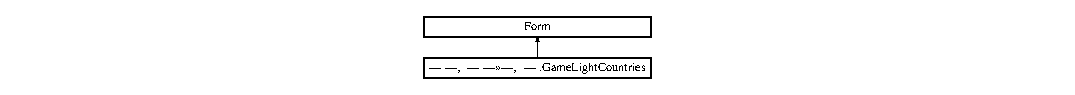
\includegraphics[height=0.824742cm]{class_xD0_x92_xD0_xB8_xD1_x81_xD0_xB5_xD0_xBB_xD0_xB8_xD1_x86_xD0_xB0_1_1_game_light_countries}
\end{center}
\end{figure}
\subsection*{Открытые члены}
\begin{DoxyCompactItemize}
\item 
\hyperlink{class_xD0_x92_xD0_xB8_xD1_x81_xD0_xB5_xD0_xBB_xD0_xB8_xD1_x86_xD0_xB0_1_1_game_light_countries_a1abbe9aa9be0d413ffed9f622798f1dc}{Game\+Light\+Countries} ()
\begin{DoxyCompactList}\small\item\em Метод инициализации \end{DoxyCompactList}\end{DoxyCompactItemize}
\subsection*{Защищенные члены}
\begin{DoxyCompactItemize}
\item 
override void \hyperlink{class_xD0_x92_xD0_xB8_xD1_x81_xD0_xB5_xD0_xBB_xD0_xB8_xD1_x86_xD0_xB0_1_1_game_light_countries_a10fdb43e2a2f0304822a77d5d799c14f}{Dispose} (bool disposing)
\begin{DoxyCompactList}\small\item\em Clean up any resources being used. \end{DoxyCompactList}\end{DoxyCompactItemize}


\subsection{Подробное описание}
Класс \hyperlink{class_xD0_x92_xD0_xB8_xD1_x81_xD0_xB5_xD0_xBB_xD0_xB8_xD1_x86_xD0_xB0_1_1_game_light_countries}{Game\+Light\+Countries}. 

Основной и единственный класс, отвечающий за окно игрового поля для лёгкого уровня категории стран 

\subsection{Конструктор(ы)}
\hypertarget{class_xD0_x92_xD0_xB8_xD1_x81_xD0_xB5_xD0_xBB_xD0_xB8_xD1_x86_xD0_xB0_1_1_game_light_countries_a1abbe9aa9be0d413ffed9f622798f1dc}{\index{Виселица\+::\+Game\+Light\+Countries@{Виселица\+::\+Game\+Light\+Countries}!Game\+Light\+Countries@{Game\+Light\+Countries}}
\index{Game\+Light\+Countries@{Game\+Light\+Countries}!Виселица\+::\+Game\+Light\+Countries@{Виселица\+::\+Game\+Light\+Countries}}
\subsubsection[{Game\+Light\+Countries}]{\setlength{\rightskip}{0pt plus 5cm}Виселица.\+Game\+Light\+Countries.\+Game\+Light\+Countries (
\begin{DoxyParamCaption}
{}
\end{DoxyParamCaption}
)\hspace{0.3cm}{\ttfamily [inline]}}}\label{class_xD0_x92_xD0_xB8_xD1_x81_xD0_xB5_xD0_xBB_xD0_xB8_xD1_x86_xD0_xB0_1_1_game_light_countries_a1abbe9aa9be0d413ffed9f622798f1dc}


Метод инициализации 

Инициализация всех компонентов окна Игровое поле лёгкого уровня категории стран 

\subsection{Методы}
\hypertarget{class_xD0_x92_xD0_xB8_xD1_x81_xD0_xB5_xD0_xBB_xD0_xB8_xD1_x86_xD0_xB0_1_1_game_light_countries_a10fdb43e2a2f0304822a77d5d799c14f}{\index{Виселица\+::\+Game\+Light\+Countries@{Виселица\+::\+Game\+Light\+Countries}!Dispose@{Dispose}}
\index{Dispose@{Dispose}!Виселица\+::\+Game\+Light\+Countries@{Виселица\+::\+Game\+Light\+Countries}}
\subsubsection[{Dispose}]{\setlength{\rightskip}{0pt plus 5cm}override void Виселица.\+Game\+Light\+Countries.\+Dispose (
\begin{DoxyParamCaption}
\item[{bool}]{disposing}
\end{DoxyParamCaption}
)\hspace{0.3cm}{\ttfamily [inline]}, {\ttfamily [protected]}}}\label{class_xD0_x92_xD0_xB8_xD1_x81_xD0_xB5_xD0_xBB_xD0_xB8_xD1_x86_xD0_xB0_1_1_game_light_countries_a10fdb43e2a2f0304822a77d5d799c14f}


Clean up any resources being used. 


\begin{DoxyParams}{Аргументы}
{\em disposing} & true if managed resources should be disposed; otherwise, false.\\
\hline
\end{DoxyParams}


Объявления и описания членов классов находятся в файлах\+:\begin{DoxyCompactItemize}
\item 
Виселица/Виселица/\hyperlink{_game_light_countries_8cs}{Game\+Light\+Countries.\+cs}\item 
Виселица/Виселица/Game\+Light\+Countries.\+Designer.\+cs\end{DoxyCompactItemize}

\hypertarget{class_xD0_x92_xD0_xB8_xD1_x81_xD0_xB5_xD0_xBB_xD0_xB8_xD1_x86_xD0_xB0_1_1_menu}{\section{Класс Виселица.\+Menu}
\label{class_xD0_x92_xD0_xB8_xD1_x81_xD0_xB5_xD0_xBB_xD0_xB8_xD1_x86_xD0_xB0_1_1_menu}\index{Виселица.\+Menu@{Виселица.\+Menu}}
}


Класс \hyperlink{class_xD0_x92_xD0_xB8_xD1_x81_xD0_xB5_xD0_xBB_xD0_xB8_xD1_x86_xD0_xB0_1_1_menu}{Menu}.  


Граф наследования\+:Виселица.\+Menu\+:\begin{figure}[H]
\begin{center}
\leavevmode
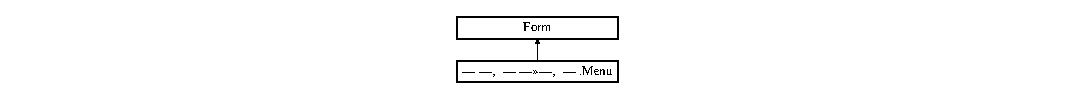
\includegraphics[height=0.877056cm]{class_xD0_x92_xD0_xB8_xD1_x81_xD0_xB5_xD0_xBB_xD0_xB8_xD1_x86_xD0_xB0_1_1_menu}
\end{center}
\end{figure}
\subsection*{Открытые члены}
\begin{DoxyCompactItemize}
\item 
\hyperlink{class_xD0_x92_xD0_xB8_xD1_x81_xD0_xB5_xD0_xBB_xD0_xB8_xD1_x86_xD0_xB0_1_1_menu_aa873418930f87a61579c8f249f5e6b61}{Menu} ()
\begin{DoxyCompactList}\small\item\em Метод инициализации \end{DoxyCompactList}\end{DoxyCompactItemize}
\subsection*{Защищенные члены}
\begin{DoxyCompactItemize}
\item 
override void \hyperlink{class_xD0_x92_xD0_xB8_xD1_x81_xD0_xB5_xD0_xBB_xD0_xB8_xD1_x86_xD0_xB0_1_1_menu_a2cfce6cff9aa9ffeb76206de2bda9dea}{Dispose} (bool disposing)
\begin{DoxyCompactList}\small\item\em Освободить все используемые ресурсы. \end{DoxyCompactList}\end{DoxyCompactItemize}


\subsection{Подробное описание}
Класс \hyperlink{class_xD0_x92_xD0_xB8_xD1_x81_xD0_xB5_xD0_xBB_xD0_xB8_xD1_x86_xD0_xB0_1_1_menu}{Menu}. 

Основной и единственный класс, отвечающий за основное меню игры 

\subsection{Конструктор(ы)}
\hypertarget{class_xD0_x92_xD0_xB8_xD1_x81_xD0_xB5_xD0_xBB_xD0_xB8_xD1_x86_xD0_xB0_1_1_menu_aa873418930f87a61579c8f249f5e6b61}{\index{Виселица\+::\+Menu@{Виселица\+::\+Menu}!Menu@{Menu}}
\index{Menu@{Menu}!Виселица\+::\+Menu@{Виселица\+::\+Menu}}
\subsubsection[{Menu}]{\setlength{\rightskip}{0pt plus 5cm}Виселица.\+Menu.\+Menu (
\begin{DoxyParamCaption}
{}
\end{DoxyParamCaption}
)\hspace{0.3cm}{\ttfamily [inline]}}}\label{class_xD0_x92_xD0_xB8_xD1_x81_xD0_xB5_xD0_xBB_xD0_xB8_xD1_x86_xD0_xB0_1_1_menu_aa873418930f87a61579c8f249f5e6b61}


Метод инициализации 

Инициализация всех компонентов окна Меню 

\subsection{Методы}
\hypertarget{class_xD0_x92_xD0_xB8_xD1_x81_xD0_xB5_xD0_xBB_xD0_xB8_xD1_x86_xD0_xB0_1_1_menu_a2cfce6cff9aa9ffeb76206de2bda9dea}{\index{Виселица\+::\+Menu@{Виселица\+::\+Menu}!Dispose@{Dispose}}
\index{Dispose@{Dispose}!Виселица\+::\+Menu@{Виселица\+::\+Menu}}
\subsubsection[{Dispose}]{\setlength{\rightskip}{0pt plus 5cm}override void Виселица.\+Menu.\+Dispose (
\begin{DoxyParamCaption}
\item[{bool}]{disposing}
\end{DoxyParamCaption}
)\hspace{0.3cm}{\ttfamily [inline]}, {\ttfamily [protected]}}}\label{class_xD0_x92_xD0_xB8_xD1_x81_xD0_xB5_xD0_xBB_xD0_xB8_xD1_x86_xD0_xB0_1_1_menu_a2cfce6cff9aa9ffeb76206de2bda9dea}


Освободить все используемые ресурсы. 


\begin{DoxyParams}{Аргументы}
{\em disposing} & истинно, если управляемый ресурс должен быть удален; иначе ложно.\\
\hline
\end{DoxyParams}


Объявления и описания членов классов находятся в файлах\+:\begin{DoxyCompactItemize}
\item 
Виселица/Виселица/\hyperlink{_menu_8cs}{Menu.\+cs}\item 
Виселица/Виселица/Menu.\+Designer.\+cs\end{DoxyCompactItemize}

\hypertarget{class_xD0_x92_xD0_xB8_xD1_x81_xD0_xB5_xD0_xBB_xD0_xB8_xD1_x86_xD0_xB0_1_1_player}{\section{Класс Виселица.\+Player}
\label{class_xD0_x92_xD0_xB8_xD1_x81_xD0_xB5_xD0_xBB_xD0_xB8_xD1_x86_xD0_xB0_1_1_player}\index{Виселица.\+Player@{Виселица.\+Player}}
}


Класс \hyperlink{class_xD0_x92_xD0_xB8_xD1_x81_xD0_xB5_xD0_xBB_xD0_xB8_xD1_x86_xD0_xB0_1_1_player}{Player}.  


Граф наследования\+:Виселица.\+Player\+:\begin{figure}[H]
\begin{center}
\leavevmode

\includegraphics[height=0.873635cm]{class_xD0_x92_xD0_xB8_xD1_x81_xD0_xB5_xD0_xBB_xD0_xB8_xD1_x86_xD0_xB0_1_1_player}
\end{center}
\end{figure}
\subsection*{Открытые члены}
\begin{DoxyCompactItemize}
\item 
\hyperlink{class_xD0_x92_xD0_xB8_xD1_x81_xD0_xB5_xD0_xBB_xD0_xB8_xD1_x86_xD0_xB0_1_1_player_a5cec4eb8abd2040b26387a4cc5021144}{Player} ()
\begin{DoxyCompactList}\small\item\em Метод инициализации \end{DoxyCompactList}\end{DoxyCompactItemize}
\subsection*{Защищенные члены}
\begin{DoxyCompactItemize}
\item 
override void \hyperlink{class_xD0_x92_xD0_xB8_xD1_x81_xD0_xB5_xD0_xBB_xD0_xB8_xD1_x86_xD0_xB0_1_1_player_a798e3b07c0fff8707479301a4472ade2}{Dispose} (bool disposing)
\begin{DoxyCompactList}\small\item\em Clean up any resources being used. \end{DoxyCompactList}\end{DoxyCompactItemize}


\subsection{Подробное описание}
Класс \hyperlink{class_xD0_x92_xD0_xB8_xD1_x81_xD0_xB5_xD0_xBB_xD0_xB8_xD1_x86_xD0_xB0_1_1_player}{Player}. 

Основной и единственный класс, отвечающий за окно авторизации пользователей 

\subsection{Конструктор(ы)}
\hypertarget{class_xD0_x92_xD0_xB8_xD1_x81_xD0_xB5_xD0_xBB_xD0_xB8_xD1_x86_xD0_xB0_1_1_player_a5cec4eb8abd2040b26387a4cc5021144}{\index{Виселица\+::\+Player@{Виселица\+::\+Player}!Player@{Player}}
\index{Player@{Player}!Виселица\+::\+Player@{Виселица\+::\+Player}}
\subsubsection[{Player}]{\setlength{\rightskip}{0pt plus 5cm}Виселица.\+Player.\+Player (
\begin{DoxyParamCaption}
{}
\end{DoxyParamCaption}
)\hspace{0.3cm}{\ttfamily [inline]}}}\label{class_xD0_x92_xD0_xB8_xD1_x81_xD0_xB5_xD0_xBB_xD0_xB8_xD1_x86_xD0_xB0_1_1_player_a5cec4eb8abd2040b26387a4cc5021144}


Метод инициализации 

Инициализация всех компонентов окна Игрок 

\subsection{Методы}
\hypertarget{class_xD0_x92_xD0_xB8_xD1_x81_xD0_xB5_xD0_xBB_xD0_xB8_xD1_x86_xD0_xB0_1_1_player_a798e3b07c0fff8707479301a4472ade2}{\index{Виселица\+::\+Player@{Виселица\+::\+Player}!Dispose@{Dispose}}
\index{Dispose@{Dispose}!Виселица\+::\+Player@{Виселица\+::\+Player}}
\subsubsection[{Dispose}]{\setlength{\rightskip}{0pt plus 5cm}override void Виселица.\+Player.\+Dispose (
\begin{DoxyParamCaption}
\item[{bool}]{disposing}
\end{DoxyParamCaption}
)\hspace{0.3cm}{\ttfamily [inline]}, {\ttfamily [protected]}}}\label{class_xD0_x92_xD0_xB8_xD1_x81_xD0_xB5_xD0_xBB_xD0_xB8_xD1_x86_xD0_xB0_1_1_player_a798e3b07c0fff8707479301a4472ade2}


Clean up any resources being used. 


\begin{DoxyParams}{Аргументы}
{\em disposing} & true if managed resources should be disposed; otherwise, false.\\
\hline
\end{DoxyParams}


Объявления и описания членов классов находятся в файлах\+:\begin{DoxyCompactItemize}
\item 
Виселица/Виселица/\hyperlink{_player_8cs}{Player.\+cs}\item 
Виселица/Виселица/Player.\+Designer.\+cs\end{DoxyCompactItemize}

\hypertarget{class_xD0_x92_xD0_xB8_xD1_x81_xD0_xB5_xD0_xBB_xD0_xB8_xD1_x86_xD0_xB0_1_1_score_board}{\section{Класс Виселица.\+Score\+Board}
\label{class_xD0_x92_xD0_xB8_xD1_x81_xD0_xB5_xD0_xBB_xD0_xB8_xD1_x86_xD0_xB0_1_1_score_board}\index{Виселица.\+Score\+Board@{Виселица.\+Score\+Board}}
}


Класс \hyperlink{class_xD0_x92_xD0_xB8_xD1_x81_xD0_xB5_xD0_xBB_xD0_xB8_xD1_x86_xD0_xB0_1_1_score_board}{Score\+Board}.  


\subsection*{Открытые статические члены}
\begin{DoxyCompactItemize}
\item 
static Dictionary$<$ string, int $>$ \hyperlink{class_xD0_x92_xD0_xB8_xD1_x81_xD0_xB5_xD0_xBB_xD0_xB8_xD1_x86_xD0_xB0_1_1_score_board_aa37747677c15754cede71ca1f463106f}{get} ()
\begin{DoxyCompactList}\small\item\em Метод сохранения информации в текстовый файл \end{DoxyCompactList}\item 
static void \hyperlink{class_xD0_x92_xD0_xB8_xD1_x81_xD0_xB5_xD0_xBB_xD0_xB8_xD1_x86_xD0_xB0_1_1_score_board_a0c72ad34ad7743d96ad87813c3e96fd1}{win} ()
\begin{DoxyCompactList}\small\item\em Метод счётчика побед \end{DoxyCompactList}\end{DoxyCompactItemize}
\subsection*{Свойства}
\begin{DoxyCompactItemize}
\item 
static string \hyperlink{class_xD0_x92_xD0_xB8_xD1_x81_xD0_xB5_xD0_xBB_xD0_xB8_xD1_x86_xD0_xB0_1_1_score_board_ad744d39c7bc2c4b7f126dfdd4c68b92c}{me}\hspace{0.3cm}{\ttfamily  \mbox{[}get, set\mbox{]}}
\begin{DoxyCompactList}\small\item\em Метод определения таблицы рекордов \end{DoxyCompactList}\end{DoxyCompactItemize}


\subsection{Подробное описание}
Класс \hyperlink{class_xD0_x92_xD0_xB8_xD1_x81_xD0_xB5_xD0_xBB_xD0_xB8_xD1_x86_xD0_xB0_1_1_score_board}{Score\+Board}. 

Основной и единственный класс, отвечающий за таблицу рекордов 

\subsection{Методы}
\hypertarget{class_xD0_x92_xD0_xB8_xD1_x81_xD0_xB5_xD0_xBB_xD0_xB8_xD1_x86_xD0_xB0_1_1_score_board_aa37747677c15754cede71ca1f463106f}{\index{Виселица\+::\+Score\+Board@{Виселица\+::\+Score\+Board}!get@{get}}
\index{get@{get}!Виселица\+::\+Score\+Board@{Виселица\+::\+Score\+Board}}
\subsubsection[{get}]{\setlength{\rightskip}{0pt plus 5cm}static Dictionary$<$string, int$>$ Виселица.\+Score\+Board.\+get (
\begin{DoxyParamCaption}
{}
\end{DoxyParamCaption}
)\hspace{0.3cm}{\ttfamily [inline]}, {\ttfamily [static]}}}\label{class_xD0_x92_xD0_xB8_xD1_x81_xD0_xB5_xD0_xBB_xD0_xB8_xD1_x86_xD0_xB0_1_1_score_board_aa37747677c15754cede71ca1f463106f}


Метод сохранения информации в текстовый файл 

Сохранение информации в файл 
\begin{DoxyParams}{Аргументы}
{\em l} & Количество побед \\
\hline
{\em name} & Имя игрока \\
\hline
\end{DoxyParams}
\hypertarget{class_xD0_x92_xD0_xB8_xD1_x81_xD0_xB5_xD0_xBB_xD0_xB8_xD1_x86_xD0_xB0_1_1_score_board_a0c72ad34ad7743d96ad87813c3e96fd1}{\index{Виселица\+::\+Score\+Board@{Виселица\+::\+Score\+Board}!win@{win}}
\index{win@{win}!Виселица\+::\+Score\+Board@{Виселица\+::\+Score\+Board}}
\subsubsection[{win}]{\setlength{\rightskip}{0pt plus 5cm}static void Виселица.\+Score\+Board.\+win (
\begin{DoxyParamCaption}
{}
\end{DoxyParamCaption}
)\hspace{0.3cm}{\ttfamily [inline]}, {\ttfamily [static]}}}\label{class_xD0_x92_xD0_xB8_xD1_x81_xD0_xB5_xD0_xBB_xD0_xB8_xD1_x86_xD0_xB0_1_1_score_board_a0c72ad34ad7743d96ad87813c3e96fd1}


Метод счётчика побед 

Счётчик побед 
\begin{DoxyParams}{Аргументы}
{\em score} & Количество побед \\
\hline
{\em me} & Определение таблицы \\
\hline
{\em arr} & Массив строк \\
\hline
{\em z} & Счётчик строк \\
\hline
\end{DoxyParams}


\subsection{Полный список свойств}
\hypertarget{class_xD0_x92_xD0_xB8_xD1_x81_xD0_xB5_xD0_xBB_xD0_xB8_xD1_x86_xD0_xB0_1_1_score_board_ad744d39c7bc2c4b7f126dfdd4c68b92c}{\index{Виселица\+::\+Score\+Board@{Виселица\+::\+Score\+Board}!me@{me}}
\index{me@{me}!Виселица\+::\+Score\+Board@{Виселица\+::\+Score\+Board}}
\subsubsection[{me}]{\setlength{\rightskip}{0pt plus 5cm}string Виселица.\+Score\+Board.\+me\hspace{0.3cm}{\ttfamily [static]}, {\ttfamily [get]}, {\ttfamily [set]}}}\label{class_xD0_x92_xD0_xB8_xD1_x81_xD0_xB5_xD0_xBB_xD0_xB8_xD1_x86_xD0_xB0_1_1_score_board_ad744d39c7bc2c4b7f126dfdd4c68b92c}


Метод определения таблицы рекордов 

Определение таблицы рекордов 
\begin{DoxyParams}{Аргументы}
{\em me} & Таблица рекордов \\
\hline
\end{DoxyParams}


Объявления и описания членов класса находятся в файле\+:\begin{DoxyCompactItemize}
\item 
Виселица/Виселица/\hyperlink{_score_board_8cs}{Score\+Board.\+cs}\end{DoxyCompactItemize}

\hypertarget{class_xD0_x92_xD0_xB8_xD1_x81_xD0_xB5_xD0_xBB_xD0_xB8_xD1_x86_xD0_xB0_1_1_spravka}{\section{Класс Виселица.\+Spravka}
\label{class_xD0_x92_xD0_xB8_xD1_x81_xD0_xB5_xD0_xBB_xD0_xB8_xD1_x86_xD0_xB0_1_1_spravka}\index{Виселица.\+Spravka@{Виселица.\+Spravka}}
}


Класс \hyperlink{class_xD0_x92_xD0_xB8_xD1_x81_xD0_xB5_xD0_xBB_xD0_xB8_xD1_x86_xD0_xB0_1_1_spravka}{Spravka}.  


Граф наследования\+:Виселица.\+Spravka\+:\begin{figure}[H]
\begin{center}
\leavevmode

\includegraphics[height=0.866873cm]{class_xD0_x92_xD0_xB8_xD1_x81_xD0_xB5_xD0_xBB_xD0_xB8_xD1_x86_xD0_xB0_1_1_spravka}
\end{center}
\end{figure}
\subsection*{Открытые члены}
\begin{DoxyCompactItemize}
\item 
\hyperlink{class_xD0_x92_xD0_xB8_xD1_x81_xD0_xB5_xD0_xBB_xD0_xB8_xD1_x86_xD0_xB0_1_1_spravka_a894952df2d5b24441ea4c59fab5a2f04}{Spravka} ()
\begin{DoxyCompactList}\small\item\em Метод инициализации \end{DoxyCompactList}\end{DoxyCompactItemize}
\subsection*{Защищенные члены}
\begin{DoxyCompactItemize}
\item 
override void \hyperlink{class_xD0_x92_xD0_xB8_xD1_x81_xD0_xB5_xD0_xBB_xD0_xB8_xD1_x86_xD0_xB0_1_1_spravka_af9b0f2ef48d257b2840ea97973929229}{Dispose} (bool disposing)
\begin{DoxyCompactList}\small\item\em Clean up any resources being used. \end{DoxyCompactList}\end{DoxyCompactItemize}


\subsection{Подробное описание}
Класс \hyperlink{class_xD0_x92_xD0_xB8_xD1_x81_xD0_xB5_xD0_xBB_xD0_xB8_xD1_x86_xD0_xB0_1_1_spravka}{Spravka}. 

Основной и единственный класс, отвечающий за окно со справкой игры 

\subsection{Конструктор(ы)}
\hypertarget{class_xD0_x92_xD0_xB8_xD1_x81_xD0_xB5_xD0_xBB_xD0_xB8_xD1_x86_xD0_xB0_1_1_spravka_a894952df2d5b24441ea4c59fab5a2f04}{\index{Виселица\+::\+Spravka@{Виселица\+::\+Spravka}!Spravka@{Spravka}}
\index{Spravka@{Spravka}!Виселица\+::\+Spravka@{Виселица\+::\+Spravka}}
\subsubsection[{Spravka}]{\setlength{\rightskip}{0pt plus 5cm}Виселица.\+Spravka.\+Spravka (
\begin{DoxyParamCaption}
{}
\end{DoxyParamCaption}
)\hspace{0.3cm}{\ttfamily [inline]}}}\label{class_xD0_x92_xD0_xB8_xD1_x81_xD0_xB5_xD0_xBB_xD0_xB8_xD1_x86_xD0_xB0_1_1_spravka_a894952df2d5b24441ea4c59fab5a2f04}


Метод инициализации 

Инициализация всех компонентов окна Справка 

\subsection{Методы}
\hypertarget{class_xD0_x92_xD0_xB8_xD1_x81_xD0_xB5_xD0_xBB_xD0_xB8_xD1_x86_xD0_xB0_1_1_spravka_af9b0f2ef48d257b2840ea97973929229}{\index{Виселица\+::\+Spravka@{Виселица\+::\+Spravka}!Dispose@{Dispose}}
\index{Dispose@{Dispose}!Виселица\+::\+Spravka@{Виселица\+::\+Spravka}}
\subsubsection[{Dispose}]{\setlength{\rightskip}{0pt plus 5cm}override void Виселица.\+Spravka.\+Dispose (
\begin{DoxyParamCaption}
\item[{bool}]{disposing}
\end{DoxyParamCaption}
)\hspace{0.3cm}{\ttfamily [inline]}, {\ttfamily [protected]}}}\label{class_xD0_x92_xD0_xB8_xD1_x81_xD0_xB5_xD0_xBB_xD0_xB8_xD1_x86_xD0_xB0_1_1_spravka_af9b0f2ef48d257b2840ea97973929229}


Clean up any resources being used. 


\begin{DoxyParams}{Аргументы}
{\em disposing} & true if managed resources should be disposed; otherwise, false.\\
\hline
\end{DoxyParams}


Объявления и описания членов классов находятся в файлах\+:\begin{DoxyCompactItemize}
\item 
Виселица/Виселица/\hyperlink{_spravka_8cs}{Spravka.\+cs}\item 
Виселица/Виселица/Spravka.\+Designer.\+cs\end{DoxyCompactItemize}

\hypertarget{class_xD0_x92_xD0_xB8_xD1_x81_xD0_xB5_xD0_xBB_xD0_xB8_xD1_x86_xD0_xB0_1_1_table}{\section{Класс Виселица.\+Table}
\label{class_xD0_x92_xD0_xB8_xD1_x81_xD0_xB5_xD0_xBB_xD0_xB8_xD1_x86_xD0_xB0_1_1_table}\index{Виселица.\+Table@{Виселица.\+Table}}
}


Класс \hyperlink{class_xD0_x92_xD0_xB8_xD1_x81_xD0_xB5_xD0_xBB_xD0_xB8_xD1_x86_xD0_xB0_1_1_table}{Table}.  


Граф наследования\+:Виселица.\+Table\+:\begin{figure}[H]
\begin{center}
\leavevmode

\includegraphics[height=0.877743cm]{class_xD0_x92_xD0_xB8_xD1_x81_xD0_xB5_xD0_xBB_xD0_xB8_xD1_x86_xD0_xB0_1_1_table}
\end{center}
\end{figure}
\subsection*{Открытые члены}
\begin{DoxyCompactItemize}
\item 
\hyperlink{class_xD0_x92_xD0_xB8_xD1_x81_xD0_xB5_xD0_xBB_xD0_xB8_xD1_x86_xD0_xB0_1_1_table_a8651db4598c9bba5f032b60b31881556}{Table} ()
\begin{DoxyCompactList}\small\item\em Метод инициализации \end{DoxyCompactList}\end{DoxyCompactItemize}
\subsection*{Защищенные члены}
\begin{DoxyCompactItemize}
\item 
override void \hyperlink{class_xD0_x92_xD0_xB8_xD1_x81_xD0_xB5_xD0_xBB_xD0_xB8_xD1_x86_xD0_xB0_1_1_table_a4e7df17f00af02118c3a3046aa270a48}{Dispose} (bool disposing)
\begin{DoxyCompactList}\small\item\em Clean up any resources being used. \end{DoxyCompactList}\end{DoxyCompactItemize}


\subsection{Подробное описание}
Класс \hyperlink{class_xD0_x92_xD0_xB8_xD1_x81_xD0_xB5_xD0_xBB_xD0_xB8_xD1_x86_xD0_xB0_1_1_table}{Table}. 

Основной и единственный класс, отвечающий за окно с таблицей лидеров 

\subsection{Конструктор(ы)}
\hypertarget{class_xD0_x92_xD0_xB8_xD1_x81_xD0_xB5_xD0_xBB_xD0_xB8_xD1_x86_xD0_xB0_1_1_table_a8651db4598c9bba5f032b60b31881556}{\index{Виселица\+::\+Table@{Виселица\+::\+Table}!Table@{Table}}
\index{Table@{Table}!Виселица\+::\+Table@{Виселица\+::\+Table}}
\subsubsection[{Table}]{\setlength{\rightskip}{0pt plus 5cm}Виселица.\+Table.\+Table (
\begin{DoxyParamCaption}
{}
\end{DoxyParamCaption}
)\hspace{0.3cm}{\ttfamily [inline]}}}\label{class_xD0_x92_xD0_xB8_xD1_x81_xD0_xB5_xD0_xBB_xD0_xB8_xD1_x86_xD0_xB0_1_1_table_a8651db4598c9bba5f032b60b31881556}


Метод инициализации 

Инициализация всех компонентов окна Таблица лидеров 

\subsection{Методы}
\hypertarget{class_xD0_x92_xD0_xB8_xD1_x81_xD0_xB5_xD0_xBB_xD0_xB8_xD1_x86_xD0_xB0_1_1_table_a4e7df17f00af02118c3a3046aa270a48}{\index{Виселица\+::\+Table@{Виселица\+::\+Table}!Dispose@{Dispose}}
\index{Dispose@{Dispose}!Виселица\+::\+Table@{Виселица\+::\+Table}}
\subsubsection[{Dispose}]{\setlength{\rightskip}{0pt plus 5cm}override void Виселица.\+Table.\+Dispose (
\begin{DoxyParamCaption}
\item[{bool}]{disposing}
\end{DoxyParamCaption}
)\hspace{0.3cm}{\ttfamily [inline]}, {\ttfamily [protected]}}}\label{class_xD0_x92_xD0_xB8_xD1_x81_xD0_xB5_xD0_xBB_xD0_xB8_xD1_x86_xD0_xB0_1_1_table_a4e7df17f00af02118c3a3046aa270a48}


Clean up any resources being used. 


\begin{DoxyParams}{Аргументы}
{\em disposing} & true if managed resources should be disposed; otherwise, false.\\
\hline
\end{DoxyParams}


Объявления и описания членов классов находятся в файлах\+:\begin{DoxyCompactItemize}
\item 
Виселица/Виселица/\hyperlink{_table_8cs}{Table.\+cs}\item 
Виселица/Виселица/Table.\+Designer.\+cs\end{DoxyCompactItemize}

\chapter{Файлы}
\hypertarget{_difficulty_animals_8cs}{\section{Файл Виселица/Виселица/\+Difficulty\+Animals.cs}
\label{_difficulty_animals_8cs}\index{Виселица/Виселица/\+Difficulty\+Animals.\+cs@{Виселица/Виселица/\+Difficulty\+Animals.\+cs}}
}


Файл окна выбора уровней сложности для категории животных  


\subsection*{Классы}
\begin{DoxyCompactItemize}
\item 
class \hyperlink{class_xD0_x92_xD0_xB8_xD1_x81_xD0_xB5_xD0_xBB_xD0_xB8_xD1_x86_xD0_xB0_1_1_difficulty_animals}{Виселица.\+Difficulty\+Animals}
\begin{DoxyCompactList}\small\item\em Класс \hyperlink{class_xD0_x92_xD0_xB8_xD1_x81_xD0_xB5_xD0_xBB_xD0_xB8_xD1_x86_xD0_xB0_1_1_difficulty_animals}{Difficulty\+Animals}. \end{DoxyCompactList}\end{DoxyCompactItemize}
\subsection*{Пространства имен}
\begin{DoxyCompactItemize}
\item 
package \hyperlink{namespace_xD0_x92_xD0_xB8_xD1_x81_xD0_xB5_xD0_xBB_xD0_xB8_xD1_x86_xD0_xB0}{Виселица}
\end{DoxyCompactItemize}


\subsection{Подробное описание}
Файл окна выбора уровней сложности для категории животных 

\begin{DoxyCopyright}{Авторство}
Viselitsa 
\end{DoxyCopyright}
\begin{DoxyAuthor}{Автор}
Соколова В.\+А. 
\end{DoxyAuthor}
\begin{DoxyDate}{Дата}
10-\/05-\/2024 
\end{DoxyDate}
\begin{DoxyVersion}{Версия}
1.\+1.\+20 
\end{DoxyVersion}
\begin{DoxyParagraph}{Использует класс\+:}
Difficulty\+Animals 
\end{DoxyParagraph}
\begin{DoxyParagraph}{Содержит класс\+:}
Difficulty\+Animals 
\end{DoxyParagraph}

\hypertarget{_difficulty_cities_8cs}{\section{Файл Виселица/Виселица/\+Difficulty\+Cities.cs}
\label{_difficulty_cities_8cs}\index{Виселица/Виселица/\+Difficulty\+Cities.\+cs@{Виселица/Виселица/\+Difficulty\+Cities.\+cs}}
}


Файл окна выбора уровней сложности для категории городов  


\subsection*{Классы}
\begin{DoxyCompactItemize}
\item 
class \hyperlink{class_xD0_x92_xD0_xB8_xD1_x81_xD0_xB5_xD0_xBB_xD0_xB8_xD1_x86_xD0_xB0_1_1_difficulty_cities}{Виселица.\+Difficulty\+Cities}
\begin{DoxyCompactList}\small\item\em Класс \hyperlink{class_xD0_x92_xD0_xB8_xD1_x81_xD0_xB5_xD0_xBB_xD0_xB8_xD1_x86_xD0_xB0_1_1_difficulty_cities}{Difficulty\+Cities}. \end{DoxyCompactList}\end{DoxyCompactItemize}
\subsection*{Пространства имен}
\begin{DoxyCompactItemize}
\item 
package \hyperlink{namespace_xD0_x92_xD0_xB8_xD1_x81_xD0_xB5_xD0_xBB_xD0_xB8_xD1_x86_xD0_xB0}{Виселица}
\end{DoxyCompactItemize}


\subsection{Подробное описание}
Файл окна выбора уровней сложности для категории городов 

\begin{DoxyCopyright}{Авторство}
Viselitsa 
\end{DoxyCopyright}
\begin{DoxyAuthor}{Автор}
Соколова В.\+А. 
\end{DoxyAuthor}
\begin{DoxyDate}{Дата}
10-\/05-\/2024 
\end{DoxyDate}
\begin{DoxyVersion}{Версия}
1.\+1.\+20 
\end{DoxyVersion}
\begin{DoxyParagraph}{Использует класс\+:}
Difficulty\+Cities 
\end{DoxyParagraph}
\begin{DoxyParagraph}{Содержит класс\+:}
Difficulty\+Cities 
\end{DoxyParagraph}

\hypertarget{_difficulty_countries_8cs}{\section{Файл Виселица/Виселица/\+Difficulty\+Countries.cs}
\label{_difficulty_countries_8cs}\index{Виселица/Виселица/\+Difficulty\+Countries.\+cs@{Виселица/Виселица/\+Difficulty\+Countries.\+cs}}
}


Файл окна выбора уровней сложности для категории стран  


\subsection*{Классы}
\begin{DoxyCompactItemize}
\item 
class \hyperlink{class_xD0_x92_xD0_xB8_xD1_x81_xD0_xB5_xD0_xBB_xD0_xB8_xD1_x86_xD0_xB0_1_1_difficulty_countries}{Виселица.\+Difficulty\+Countries}
\begin{DoxyCompactList}\small\item\em Класс \hyperlink{class_xD0_x92_xD0_xB8_xD1_x81_xD0_xB5_xD0_xBB_xD0_xB8_xD1_x86_xD0_xB0_1_1_difficulty_countries}{Difficulty\+Countries}. \end{DoxyCompactList}\end{DoxyCompactItemize}
\subsection*{Пространства имен}
\begin{DoxyCompactItemize}
\item 
package \hyperlink{namespace_xD0_x92_xD0_xB8_xD1_x81_xD0_xB5_xD0_xBB_xD0_xB8_xD1_x86_xD0_xB0}{Виселица}
\end{DoxyCompactItemize}


\subsection{Подробное описание}
Файл окна выбора уровней сложности для категории стран 

\begin{DoxyCopyright}{Авторство}
Viselitsa 
\end{DoxyCopyright}
\begin{DoxyAuthor}{Автор}
Соколова В.\+А. 
\end{DoxyAuthor}
\begin{DoxyDate}{Дата}
10-\/05-\/2024 
\end{DoxyDate}
\begin{DoxyVersion}{Версия}
1.\+1.\+20 
\end{DoxyVersion}
\begin{DoxyParagraph}{Использует класс\+:}
Difficulty\+Countries 
\end{DoxyParagraph}
\begin{DoxyParagraph}{Содержит класс\+:}
Difficulty\+Countries 
\end{DoxyParagraph}

\hypertarget{_game_average_animals_8cs}{\section{Файл Виселица/Виселица/\+Game\+Average\+Animals.cs}
\label{_game_average_animals_8cs}\index{Виселица/Виселица/\+Game\+Average\+Animals.\+cs@{Виселица/Виселица/\+Game\+Average\+Animals.\+cs}}
}


Файл окна игрового поля для среднего уровня категории животных  


\subsection*{Классы}
\begin{DoxyCompactItemize}
\item 
class \hyperlink{class_xD0_x92_xD0_xB8_xD1_x81_xD0_xB5_xD0_xBB_xD0_xB8_xD1_x86_xD0_xB0_1_1_game_average_animals}{Виселица.\+Game\+Average\+Animals}
\begin{DoxyCompactList}\small\item\em Класс \hyperlink{class_xD0_x92_xD0_xB8_xD1_x81_xD0_xB5_xD0_xBB_xD0_xB8_xD1_x86_xD0_xB0_1_1_game_average_animals}{Game\+Average\+Animals}. \end{DoxyCompactList}\end{DoxyCompactItemize}
\subsection*{Пространства имен}
\begin{DoxyCompactItemize}
\item 
package \hyperlink{namespace_xD0_x92_xD0_xB8_xD1_x81_xD0_xB5_xD0_xBB_xD0_xB8_xD1_x86_xD0_xB0}{Виселица}
\end{DoxyCompactItemize}


\subsection{Подробное описание}
Файл окна игрового поля для среднего уровня категории животных 

\begin{DoxyCopyright}{Авторство}
Viselitsa 
\end{DoxyCopyright}
\begin{DoxyAuthor}{Автор}
Соколова В.\+А. 
\end{DoxyAuthor}
\begin{DoxyDate}{Дата}
10-\/05-\/2024 
\end{DoxyDate}
\begin{DoxyVersion}{Версия}
1.\+1.\+20 
\end{DoxyVersion}
\begin{DoxyParagraph}{Использует класс\+:}
Game\+Average\+Animals 
\end{DoxyParagraph}
\begin{DoxyParagraph}{Содержит класс\+:}
Game\+Average\+Animals 
\end{DoxyParagraph}

\hypertarget{_game_average_cities_8cs}{\section{Файл Виселица/Виселица/\+Game\+Average\+Cities.cs}
\label{_game_average_cities_8cs}\index{Виселица/Виселица/\+Game\+Average\+Cities.\+cs@{Виселица/Виселица/\+Game\+Average\+Cities.\+cs}}
}


Файл окна игрового поля для среднего уровня категории городов  


\subsection*{Классы}
\begin{DoxyCompactItemize}
\item 
class \hyperlink{class_xD0_x92_xD0_xB8_xD1_x81_xD0_xB5_xD0_xBB_xD0_xB8_xD1_x86_xD0_xB0_1_1_game_average_cities}{Виселица.\+Game\+Average\+Cities}
\begin{DoxyCompactList}\small\item\em Класс \hyperlink{class_xD0_x92_xD0_xB8_xD1_x81_xD0_xB5_xD0_xBB_xD0_xB8_xD1_x86_xD0_xB0_1_1_game_average_cities}{Game\+Average\+Cities}. \end{DoxyCompactList}\end{DoxyCompactItemize}
\subsection*{Пространства имен}
\begin{DoxyCompactItemize}
\item 
package \hyperlink{namespace_xD0_x92_xD0_xB8_xD1_x81_xD0_xB5_xD0_xBB_xD0_xB8_xD1_x86_xD0_xB0}{Виселица}
\end{DoxyCompactItemize}


\subsection{Подробное описание}
Файл окна игрового поля для среднего уровня категории городов 

\begin{DoxyCopyright}{Авторство}
Viselitsa 
\end{DoxyCopyright}
\begin{DoxyAuthor}{Автор}
Соколова В.\+А. 
\end{DoxyAuthor}
\begin{DoxyDate}{Дата}
10-\/05-\/2024 
\end{DoxyDate}
\begin{DoxyVersion}{Версия}
1.\+1.\+20 
\end{DoxyVersion}
\begin{DoxyParagraph}{Использует класс\+:}
Game\+Average\+Cities 
\end{DoxyParagraph}
\begin{DoxyParagraph}{Содержит класс\+:}
Game\+Average\+Cities 
\end{DoxyParagraph}

\hypertarget{_game_average_countries_8cs}{\section{Файл Виселица/Виселица/\+Game\+Average\+Countries.cs}
\label{_game_average_countries_8cs}\index{Виселица/Виселица/\+Game\+Average\+Countries.\+cs@{Виселица/Виселица/\+Game\+Average\+Countries.\+cs}}
}


Файл окна игрового поля для среднего уровня категории стран  


\subsection*{Классы}
\begin{DoxyCompactItemize}
\item 
class \hyperlink{class_xD0_x92_xD0_xB8_xD1_x81_xD0_xB5_xD0_xBB_xD0_xB8_xD1_x86_xD0_xB0_1_1_game_average_countries}{Виселица.\+Game\+Average\+Countries}
\begin{DoxyCompactList}\small\item\em Класс \hyperlink{class_xD0_x92_xD0_xB8_xD1_x81_xD0_xB5_xD0_xBB_xD0_xB8_xD1_x86_xD0_xB0_1_1_game_average_countries}{Game\+Average\+Countries}. \end{DoxyCompactList}\end{DoxyCompactItemize}
\subsection*{Пространства имен}
\begin{DoxyCompactItemize}
\item 
package \hyperlink{namespace_xD0_x92_xD0_xB8_xD1_x81_xD0_xB5_xD0_xBB_xD0_xB8_xD1_x86_xD0_xB0}{Виселица}
\end{DoxyCompactItemize}


\subsection{Подробное описание}
Файл окна игрового поля для среднего уровня категории стран 

\begin{DoxyCopyright}{Авторство}
Viselitsa 
\end{DoxyCopyright}
\begin{DoxyAuthor}{Автор}
Соколова В.\+А. 
\end{DoxyAuthor}
\begin{DoxyDate}{Дата}
10-\/05-\/2024 
\end{DoxyDate}
\begin{DoxyVersion}{Версия}
1.\+1.\+20 
\end{DoxyVersion}
\begin{DoxyParagraph}{Использует класс\+:}
Game\+Average\+Countries 
\end{DoxyParagraph}
\begin{DoxyParagraph}{Содержит класс\+:}
Game\+Average\+Countries 
\end{DoxyParagraph}

\hypertarget{_game_difficult_animals_8cs}{\section{Файл Виселица/Виселица/\+Game\+Difficult\+Animals.cs}
\label{_game_difficult_animals_8cs}\index{Виселица/Виселица/\+Game\+Difficult\+Animals.\+cs@{Виселица/Виселица/\+Game\+Difficult\+Animals.\+cs}}
}


Файл окна игрового поля для сложного уровня категории животных  


\subsection*{Классы}
\begin{DoxyCompactItemize}
\item 
class \hyperlink{class_xD0_x92_xD0_xB8_xD1_x81_xD0_xB5_xD0_xBB_xD0_xB8_xD1_x86_xD0_xB0_1_1_game_difficult_animals}{Виселица.\+Game\+Difficult\+Animals}
\begin{DoxyCompactList}\small\item\em Класс \hyperlink{class_xD0_x92_xD0_xB8_xD1_x81_xD0_xB5_xD0_xBB_xD0_xB8_xD1_x86_xD0_xB0_1_1_game_difficult_animals}{Game\+Difficult\+Animals}. \end{DoxyCompactList}\end{DoxyCompactItemize}
\subsection*{Пространства имен}
\begin{DoxyCompactItemize}
\item 
package \hyperlink{namespace_xD0_x92_xD0_xB8_xD1_x81_xD0_xB5_xD0_xBB_xD0_xB8_xD1_x86_xD0_xB0}{Виселица}
\end{DoxyCompactItemize}


\subsection{Подробное описание}
Файл окна игрового поля для сложного уровня категории животных 

\begin{DoxyCopyright}{Авторство}
Viselitsa 
\end{DoxyCopyright}
\begin{DoxyAuthor}{Автор}
Соколова В.\+А. 
\end{DoxyAuthor}
\begin{DoxyDate}{Дата}
10-\/05-\/2024 
\end{DoxyDate}
\begin{DoxyVersion}{Версия}
1.\+1.\+20 
\end{DoxyVersion}
\begin{DoxyParagraph}{Использует класс\+:}
Game\+Difficult\+Animals 
\end{DoxyParagraph}
\begin{DoxyParagraph}{Содержит класс\+:}
Game\+Difficult\+Animals 
\end{DoxyParagraph}

\hypertarget{_game_difficult_cities_8cs}{\section{Файл Виселица/Виселица/\+Game\+Difficult\+Cities.cs}
\label{_game_difficult_cities_8cs}\index{Виселица/Виселица/\+Game\+Difficult\+Cities.\+cs@{Виселица/Виселица/\+Game\+Difficult\+Cities.\+cs}}
}


Файл окна игрового поля для сложного уровня категории городов  


\subsection*{Классы}
\begin{DoxyCompactItemize}
\item 
class \hyperlink{class_xD0_x92_xD0_xB8_xD1_x81_xD0_xB5_xD0_xBB_xD0_xB8_xD1_x86_xD0_xB0_1_1_game_difficult_cities}{Виселица.\+Game\+Difficult\+Cities}
\begin{DoxyCompactList}\small\item\em Класс \hyperlink{class_xD0_x92_xD0_xB8_xD1_x81_xD0_xB5_xD0_xBB_xD0_xB8_xD1_x86_xD0_xB0_1_1_game_difficult_cities}{Game\+Difficult\+Cities}. \end{DoxyCompactList}\end{DoxyCompactItemize}
\subsection*{Пространства имен}
\begin{DoxyCompactItemize}
\item 
package \hyperlink{namespace_xD0_x92_xD0_xB8_xD1_x81_xD0_xB5_xD0_xBB_xD0_xB8_xD1_x86_xD0_xB0}{Виселица}
\end{DoxyCompactItemize}


\subsection{Подробное описание}
Файл окна игрового поля для сложного уровня категории городов 

\begin{DoxyCopyright}{Авторство}
Viselitsa 
\end{DoxyCopyright}
\begin{DoxyAuthor}{Автор}
Соколова В.\+А. 
\end{DoxyAuthor}
\begin{DoxyDate}{Дата}
10-\/05-\/2024 
\end{DoxyDate}
\begin{DoxyVersion}{Версия}
1.\+1.\+20 
\end{DoxyVersion}
\begin{DoxyParagraph}{Использует класс\+:}
Game\+Difficult\+Cities 
\end{DoxyParagraph}
\begin{DoxyParagraph}{Содержит класс\+:}
Game\+Difficult\+Cities 
\end{DoxyParagraph}

\hypertarget{_game_difficult_countries_8cs}{\section{Файл Виселица/Виселица/\+Game\+Difficult\+Countries.cs}
\label{_game_difficult_countries_8cs}\index{Виселица/Виселица/\+Game\+Difficult\+Countries.\+cs@{Виселица/Виселица/\+Game\+Difficult\+Countries.\+cs}}
}


Файл окна игрового поля для сложного уровня категории стран  


\subsection*{Классы}
\begin{DoxyCompactItemize}
\item 
class \hyperlink{class_xD0_x92_xD0_xB8_xD1_x81_xD0_xB5_xD0_xBB_xD0_xB8_xD1_x86_xD0_xB0_1_1_game_difficult_countries}{Виселица.\+Game\+Difficult\+Countries}
\begin{DoxyCompactList}\small\item\em Класс \hyperlink{class_xD0_x92_xD0_xB8_xD1_x81_xD0_xB5_xD0_xBB_xD0_xB8_xD1_x86_xD0_xB0_1_1_game_difficult_countries}{Game\+Difficult\+Countries}. \end{DoxyCompactList}\end{DoxyCompactItemize}
\subsection*{Пространства имен}
\begin{DoxyCompactItemize}
\item 
package \hyperlink{namespace_xD0_x92_xD0_xB8_xD1_x81_xD0_xB5_xD0_xBB_xD0_xB8_xD1_x86_xD0_xB0}{Виселица}
\end{DoxyCompactItemize}


\subsection{Подробное описание}
Файл окна игрового поля для сложного уровня категории стран 

\begin{DoxyCopyright}{Авторство}
Viselitsa 
\end{DoxyCopyright}
\begin{DoxyAuthor}{Автор}
Соколова В.\+А. 
\end{DoxyAuthor}
\begin{DoxyDate}{Дата}
10-\/05-\/2024 
\end{DoxyDate}
\begin{DoxyVersion}{Версия}
1.\+1.\+20 
\end{DoxyVersion}
\begin{DoxyParagraph}{Использует класс\+:}
Game\+Difficult\+Countries 
\end{DoxyParagraph}
\begin{DoxyParagraph}{Содержит класс\+:}
Game\+Difficult\+Countries 
\end{DoxyParagraph}

\hypertarget{_game_light_animals_8cs}{\section{Файл Виселица/Виселица/\+Game\+Light\+Animals.cs}
\label{_game_light_animals_8cs}\index{Виселица/Виселица/\+Game\+Light\+Animals.\+cs@{Виселица/Виселица/\+Game\+Light\+Animals.\+cs}}
}


Файл окна игрового поля для лёгкого уровня категории животных  


\subsection*{Классы}
\begin{DoxyCompactItemize}
\item 
class \hyperlink{class_xD0_x92_xD0_xB8_xD1_x81_xD0_xB5_xD0_xBB_xD0_xB8_xD1_x86_xD0_xB0_1_1_game_light_animals}{Виселица.\+Game\+Light\+Animals}
\begin{DoxyCompactList}\small\item\em Класс \hyperlink{class_xD0_x92_xD0_xB8_xD1_x81_xD0_xB5_xD0_xBB_xD0_xB8_xD1_x86_xD0_xB0_1_1_game_light_animals}{Game\+Light\+Animals}. \end{DoxyCompactList}\end{DoxyCompactItemize}
\subsection*{Пространства имен}
\begin{DoxyCompactItemize}
\item 
package \hyperlink{namespace_xD0_x92_xD0_xB8_xD1_x81_xD0_xB5_xD0_xBB_xD0_xB8_xD1_x86_xD0_xB0}{Виселица}
\end{DoxyCompactItemize}


\subsection{Подробное описание}
Файл окна игрового поля для лёгкого уровня категории животных 

\begin{DoxyCopyright}{Авторство}
Viselitsa 
\end{DoxyCopyright}
\begin{DoxyAuthor}{Автор}
Соколова В.\+А. 
\end{DoxyAuthor}
\begin{DoxyDate}{Дата}
10-\/05-\/2024 
\end{DoxyDate}
\begin{DoxyVersion}{Версия}
1.\+1.\+20 
\end{DoxyVersion}
\begin{DoxyParagraph}{Использует класс\+:}
Game\+Light\+Animals 
\end{DoxyParagraph}
\begin{DoxyParagraph}{Содержит класс\+:}
Game\+Light\+Animals 
\end{DoxyParagraph}

\hypertarget{_game_light_cities_8cs}{\section{Файл Виселица/Виселица/\+Game\+Light\+Cities.cs}
\label{_game_light_cities_8cs}\index{Виселица/Виселица/\+Game\+Light\+Cities.\+cs@{Виселица/Виселица/\+Game\+Light\+Cities.\+cs}}
}


Файл окна игрового поля для лёгкого уровня категории городов  


\subsection*{Классы}
\begin{DoxyCompactItemize}
\item 
class \hyperlink{class_xD0_x92_xD0_xB8_xD1_x81_xD0_xB5_xD0_xBB_xD0_xB8_xD1_x86_xD0_xB0_1_1_game_light_cities}{Виселица.\+Game\+Light\+Cities}
\begin{DoxyCompactList}\small\item\em Класс \hyperlink{class_xD0_x92_xD0_xB8_xD1_x81_xD0_xB5_xD0_xBB_xD0_xB8_xD1_x86_xD0_xB0_1_1_game_light_cities}{Game\+Light\+Cities}. \end{DoxyCompactList}\end{DoxyCompactItemize}
\subsection*{Пространства имен}
\begin{DoxyCompactItemize}
\item 
package \hyperlink{namespace_xD0_x92_xD0_xB8_xD1_x81_xD0_xB5_xD0_xBB_xD0_xB8_xD1_x86_xD0_xB0}{Виселица}
\end{DoxyCompactItemize}


\subsection{Подробное описание}
Файл окна игрового поля для лёгкого уровня категории городов 

\begin{DoxyCopyright}{Авторство}
Viselitsa 
\end{DoxyCopyright}
\begin{DoxyAuthor}{Автор}
Соколова В.\+А. 
\end{DoxyAuthor}
\begin{DoxyDate}{Дата}
10-\/05-\/2024 
\end{DoxyDate}
\begin{DoxyVersion}{Версия}
1.\+1.\+20 
\end{DoxyVersion}
\begin{DoxyParagraph}{Использует класс\+:}
Game\+Light\+Cities 
\end{DoxyParagraph}
\begin{DoxyParagraph}{Содержит класс\+:}
Game\+Light\+Cities 
\end{DoxyParagraph}

\hypertarget{_game_light_countries_8cs}{\section{Файл Виселица/Виселица/\+Game\+Light\+Countries.cs}
\label{_game_light_countries_8cs}\index{Виселица/Виселица/\+Game\+Light\+Countries.\+cs@{Виселица/Виселица/\+Game\+Light\+Countries.\+cs}}
}


Файл окна игрового поля для лёгкого уровня категории стран  


\subsection*{Классы}
\begin{DoxyCompactItemize}
\item 
class \hyperlink{class_xD0_x92_xD0_xB8_xD1_x81_xD0_xB5_xD0_xBB_xD0_xB8_xD1_x86_xD0_xB0_1_1_game_light_countries}{Виселица.\+Game\+Light\+Countries}
\begin{DoxyCompactList}\small\item\em Класс \hyperlink{class_xD0_x92_xD0_xB8_xD1_x81_xD0_xB5_xD0_xBB_xD0_xB8_xD1_x86_xD0_xB0_1_1_game_light_countries}{Game\+Light\+Countries}. \end{DoxyCompactList}\end{DoxyCompactItemize}
\subsection*{Пространства имен}
\begin{DoxyCompactItemize}
\item 
package \hyperlink{namespace_xD0_x92_xD0_xB8_xD1_x81_xD0_xB5_xD0_xBB_xD0_xB8_xD1_x86_xD0_xB0}{Виселица}
\end{DoxyCompactItemize}


\subsection{Подробное описание}
Файл окна игрового поля для лёгкого уровня категории стран 

\begin{DoxyCopyright}{Авторство}
Viselitsa 
\end{DoxyCopyright}
\begin{DoxyAuthor}{Автор}
Соколова В.\+А. 
\end{DoxyAuthor}
\begin{DoxyDate}{Дата}
10-\/05-\/2024 
\end{DoxyDate}
\begin{DoxyVersion}{Версия}
1.\+1.\+20 
\end{DoxyVersion}
\begin{DoxyParagraph}{Использует класс\+:}
Game\+Light\+Countries 
\end{DoxyParagraph}
\begin{DoxyParagraph}{Содержит класс\+:}
Game\+Light\+Countries 
\end{DoxyParagraph}

\hypertarget{_menu_8cs}{\section{Файл Виселица/Виселица/\+Menu.cs}
\label{_menu_8cs}\index{Виселица/Виселица/\+Menu.\+cs@{Виселица/Виселица/\+Menu.\+cs}}
}


Файл основного меню игры  


\subsection*{Классы}
\begin{DoxyCompactItemize}
\item 
class \hyperlink{class_xD0_x92_xD0_xB8_xD1_x81_xD0_xB5_xD0_xBB_xD0_xB8_xD1_x86_xD0_xB0_1_1_menu}{Виселица.\+Menu}
\begin{DoxyCompactList}\small\item\em Класс \hyperlink{class_xD0_x92_xD0_xB8_xD1_x81_xD0_xB5_xD0_xBB_xD0_xB8_xD1_x86_xD0_xB0_1_1_menu}{Menu}. \end{DoxyCompactList}\end{DoxyCompactItemize}
\subsection*{Пространства имен}
\begin{DoxyCompactItemize}
\item 
package \hyperlink{namespace_xD0_x92_xD0_xB8_xD1_x81_xD0_xB5_xD0_xBB_xD0_xB8_xD1_x86_xD0_xB0}{Виселица}
\end{DoxyCompactItemize}


\subsection{Подробное описание}
Файл основного меню игры 

\begin{DoxyCopyright}{Авторство}
Viselitsa 
\end{DoxyCopyright}
\begin{DoxyAuthor}{Автор}
Соколова В.\+А. 
\end{DoxyAuthor}
\begin{DoxyDate}{Дата}
10-\/05-\/2024 
\end{DoxyDate}
\begin{DoxyVersion}{Версия}
1.\+1.\+20 
\end{DoxyVersion}
\begin{DoxyParagraph}{Использует класс\+:}
Menu 
\end{DoxyParagraph}
\begin{DoxyParagraph}{Содержит класс\+:}
Menu 
\end{DoxyParagraph}

\hypertarget{_player_8cs}{\section{Файл Виселица/Виселица/\+Player.cs}
\label{_player_8cs}\index{Виселица/Виселица/\+Player.\+cs@{Виселица/Виселица/\+Player.\+cs}}
}


Файл авторизации пользователей  


\subsection*{Классы}
\begin{DoxyCompactItemize}
\item 
class \hyperlink{class_xD0_x92_xD0_xB8_xD1_x81_xD0_xB5_xD0_xBB_xD0_xB8_xD1_x86_xD0_xB0_1_1_player}{Виселица.\+Player}
\begin{DoxyCompactList}\small\item\em Класс \hyperlink{class_xD0_x92_xD0_xB8_xD1_x81_xD0_xB5_xD0_xBB_xD0_xB8_xD1_x86_xD0_xB0_1_1_player}{Player}. \end{DoxyCompactList}\end{DoxyCompactItemize}
\subsection*{Пространства имен}
\begin{DoxyCompactItemize}
\item 
package \hyperlink{namespace_xD0_x92_xD0_xB8_xD1_x81_xD0_xB5_xD0_xBB_xD0_xB8_xD1_x86_xD0_xB0}{Виселица}
\end{DoxyCompactItemize}


\subsection{Подробное описание}
Файл авторизации пользователей 

\begin{DoxyCopyright}{Авторство}
Viselitsa 
\end{DoxyCopyright}
\begin{DoxyAuthor}{Автор}
Соколова В.\+А. 
\end{DoxyAuthor}
\begin{DoxyDate}{Дата}
10-\/05-\/2024 
\end{DoxyDate}
\begin{DoxyVersion}{Версия}
1.\+1.\+20 
\end{DoxyVersion}
\begin{DoxyParagraph}{Использует класс\+:}
Player 
\end{DoxyParagraph}
\begin{DoxyParagraph}{Содержит класс\+:}
Player 
\end{DoxyParagraph}

\hypertarget{_score_board_8cs}{\section{Файл Виселица/Виселица/\+Score\+Board.cs}
\label{_score_board_8cs}\index{Виселица/Виселица/\+Score\+Board.\+cs@{Виселица/Виселица/\+Score\+Board.\+cs}}
}


Файл таблицы рекордов  


\subsection*{Классы}
\begin{DoxyCompactItemize}
\item 
class \hyperlink{class_xD0_x92_xD0_xB8_xD1_x81_xD0_xB5_xD0_xBB_xD0_xB8_xD1_x86_xD0_xB0_1_1_score_board}{Виселица.\+Score\+Board}
\begin{DoxyCompactList}\small\item\em Класс \hyperlink{class_xD0_x92_xD0_xB8_xD1_x81_xD0_xB5_xD0_xBB_xD0_xB8_xD1_x86_xD0_xB0_1_1_score_board}{Score\+Board}. \end{DoxyCompactList}\end{DoxyCompactItemize}
\subsection*{Пространства имен}
\begin{DoxyCompactItemize}
\item 
package \hyperlink{namespace_xD0_x92_xD0_xB8_xD1_x81_xD0_xB5_xD0_xBB_xD0_xB8_xD1_x86_xD0_xB0}{Виселица}
\end{DoxyCompactItemize}


\subsection{Подробное описание}
Файл таблицы рекордов 

\begin{DoxyCopyright}{Авторство}
Viselitsa 
\end{DoxyCopyright}
\begin{DoxyAuthor}{Автор}
Соколова В.\+А. 
\end{DoxyAuthor}
\begin{DoxyDate}{Дата}
10-\/05-\/2024 
\end{DoxyDate}
\begin{DoxyVersion}{Версия}
1.\+1.\+20 
\end{DoxyVersion}
\begin{DoxyParagraph}{Использует класс\+:}
Score\+Board 
\end{DoxyParagraph}
\begin{DoxyParagraph}{Содержит класс\+:}
Score\+Board 
\end{DoxyParagraph}

\hypertarget{_spravka_8cs}{\section{Файл Виселица/Виселица/\+Spravka.cs}
\label{_spravka_8cs}\index{Виселица/Виселица/\+Spravka.\+cs@{Виселица/Виселица/\+Spravka.\+cs}}
}


Файл справки игры  


\subsection*{Классы}
\begin{DoxyCompactItemize}
\item 
class \hyperlink{class_xD0_x92_xD0_xB8_xD1_x81_xD0_xB5_xD0_xBB_xD0_xB8_xD1_x86_xD0_xB0_1_1_spravka}{Виселица.\+Spravka}
\begin{DoxyCompactList}\small\item\em Класс \hyperlink{class_xD0_x92_xD0_xB8_xD1_x81_xD0_xB5_xD0_xBB_xD0_xB8_xD1_x86_xD0_xB0_1_1_spravka}{Spravka}. \end{DoxyCompactList}\end{DoxyCompactItemize}
\subsection*{Пространства имен}
\begin{DoxyCompactItemize}
\item 
package \hyperlink{namespace_xD0_x92_xD0_xB8_xD1_x81_xD0_xB5_xD0_xBB_xD0_xB8_xD1_x86_xD0_xB0}{Виселица}
\end{DoxyCompactItemize}


\subsection{Подробное описание}
Файл справки игры 

\begin{DoxyCopyright}{Авторство}
Viselitsa 
\end{DoxyCopyright}
\begin{DoxyAuthor}{Автор}
Соколова В.\+А. 
\end{DoxyAuthor}
\begin{DoxyDate}{Дата}
10-\/05-\/2024 
\end{DoxyDate}
\begin{DoxyVersion}{Версия}
1.\+1.\+20 
\end{DoxyVersion}
\begin{DoxyParagraph}{Использует класс\+:}
Spravka 
\end{DoxyParagraph}
\begin{DoxyParagraph}{Содержит класс\+:}
Spravka 
\end{DoxyParagraph}

\hypertarget{_table_8cs}{\section{Файл Виселица/Виселица/\+Table.cs}
\label{_table_8cs}\index{Виселица/Виселица/\+Table.\+cs@{Виселица/Виселица/\+Table.\+cs}}
}


Файл таблицы лидеров  


\subsection*{Классы}
\begin{DoxyCompactItemize}
\item 
class \hyperlink{class_xD0_x92_xD0_xB8_xD1_x81_xD0_xB5_xD0_xBB_xD0_xB8_xD1_x86_xD0_xB0_1_1_table}{Виселица.\+Table}
\begin{DoxyCompactList}\small\item\em Класс \hyperlink{class_xD0_x92_xD0_xB8_xD1_x81_xD0_xB5_xD0_xBB_xD0_xB8_xD1_x86_xD0_xB0_1_1_table}{Table}. \end{DoxyCompactList}\end{DoxyCompactItemize}
\subsection*{Пространства имен}
\begin{DoxyCompactItemize}
\item 
package \hyperlink{namespace_xD0_x92_xD0_xB8_xD1_x81_xD0_xB5_xD0_xBB_xD0_xB8_xD1_x86_xD0_xB0}{Виселица}
\end{DoxyCompactItemize}


\subsection{Подробное описание}
Файл таблицы лидеров 

\begin{DoxyCopyright}{Авторство}
Viselitsa 
\end{DoxyCopyright}
\begin{DoxyAuthor}{Автор}
Соколова В.\+А. 
\end{DoxyAuthor}
\begin{DoxyDate}{Дата}
10-\/05-\/2024 
\end{DoxyDate}
\begin{DoxyVersion}{Версия}
1.\+1.\+20 
\end{DoxyVersion}
\begin{DoxyParagraph}{Использует класс\+:}
Table 
\end{DoxyParagraph}
\begin{DoxyParagraph}{Содержит класс\+:}
Table 
\end{DoxyParagraph}

%--- End generated contents ---

% Index
\newpage
\phantomsection
\addcontentsline{toc}{chapter}{Алфавитный указатель}
\printindex

\end{document}
